\documentclass{template/openetcs_article}
% Use the option "nocc" if the document is not licensed under Creative Commons
%\documentclass[nocc]{template/openetcs_article} 
\usepackage{lipsum,url}
\usepackage{xspace}
\usepackage{graphicx}
\usepackage{fixme}
\usepackage{lscape} 
\usepackage{pgfgantt}
\usepackage{adjustbox}
\usepackage{datetime}
\usepackage{url}
\usepackage{amsmath}
\usepackage{algorithm}
\usepackage{hyperref}
\usepackage{tikz}
\usetikzlibrary{arrows,automata}
\usepackage{hyperref}
\usepackage{booktabs}
\graphicspath{{schema/}}
\usepackage{amsfonts}
\definecolor{hblue}{RGB}{79,129,189}

%user specified macros


\newcommand{\VV}{Verification \& Validation\xspace}
\newcommand{\vv}{verification \& validation\xspace}

\def\CC{{C\nolinebreak[4]\hspace{-.05em}\raisebox{.4ex}{\tiny\bf ++}}}

\newcommand{\bitwalker}{\mbox{\texttt{Bitwalker}}\xspace}

\newcommand{\poke}{\mbox{\texttt{Bitwalker\_Poke}}\xspace}
\newcommand{\peek}{\mbox{\texttt{Bitwalker\_Peek}}\xspace}
\newcommand{\acsl}{\mbox{\textsf{ACSL}}\xspace}
\newcommand{\isoc}{\mbox{\textsf{C}}\xspace}
\newcommand{\framac}{\mbox{\textsf{Frama-C}}\xspace}
\newcommand{\framacwp}{\mbox{\textsf{Frama-C\slash WP}}\xspace}
\newcommand{\why}{\mbox{\textsf{Why}}\xspace}
\newcommand{\wpframac}{\mbox{\textsf{WP}}\xspace}
\newcommand{\altergo}{\mbox{\textsf{Alt-Ergo}}\xspace}
\newcommand{\qed}{\mbox{\textsf{Qed}}\xspace}
\newcommand{\cvc}{\mbox{\textsf{CVC4}}\xspace}
\newcommand{\z}{\mbox{\textsf{Z3}}\xspace}
\newcommand{\coq}{\mbox{\textsf{Coq}}\xspace}
\newcommand{\cealist}{\mbox{\textsf{CEA LIST}}\xspace}

\newcommand{\inl}[1]{\lstinline[style=inline]{#1}}




\graphicspath{{./template/}{.}{./images/}}
\begin{document}
\frontmatter
\project{openETCS}

%Please do not change anything above this line
%============================
% The document metadata is defined below

\reportnum{OETCS/WP4/D4.2.1}

%define your workpackage or task here
\wp{openETCS@ITEA Work Package 4.2: ``Verification \& Validation of the Formal Model''}

%set a title here
\title{D.4.2.1 1st interim V\&V report on the applicability of the V\&V approach to the formal abstract model}

%set a subtitle here
\subtitle{}

%set the date of the report here
\date{January 2014}

%define a list of authors and their affiliation here
\author{Ana Cavalli \and João Santos}

\affiliation{Télécom SudParis\\
  9 rue Charles Fourier\\
  91011 Evry Cedex, France}
  
\author{Stefan Rieger}

\affiliation{TWT GmbH Science \& Inovation}

\author{Cécile Braunstein}
\affiliation{Uni Bremen}
  
\author{Uwe Steinke}
\affiliation{Siemens}

\author{Benoît~Lucet \and Matthias Güdemann \and Brice~Gombault \and Marielle~Petit-Doche} 

\affiliation{Systerel}

\author{Alexander Nitsch \& Benjamin Beichler}

\affiliation{University of Rostock}
  
% define the coverart
\coverart[width=350pt]{openETCS_EUPL}

%define the type of report
\reporttype{}



%\begin{abstract}
%define an abstract here

%\lipsum[12-13]

%\end{abstract}

%=============================
%Do not change the next three lines
\maketitle
\tableofcontents
\listoffiguresandtables
\newpage
%=============================

% The actual document starts below this line
%=============================


%Start here

\section*{Introduction}

To ensure the correctness and consistency of a model and its implementation, the validation
and verification has to be performed alongside with the modelling process. Thus these tasks will
be performed repeatedly during WP3 and will provide feedback to it.

This document presents the results of the first iteration of verification and validation of the formal model. This was be accomplished
by applying the methods chosen in WP4 Task 1 onto the formal model using the tool
chain developed in WP7. 

This deliverable is a result of the contribution from different partners from the project. The following sections present the contributions of the partners.

\section{Institut Mines-Télécom}

\subsection{Model Based on Extended Timed Finite State Machines}

Over the past century, Europe's railways have been developed within national boundaries, resulting in a variety of different signaling and train control systems, which hampers cross-border traffic. In order to increase interoperability for the railway sector, the European Union has decided to adopt and standardize the European Train Control System (ETCS) new methods and tools to verify the reliability of such system need to be elaborated. Therefore, new techniques for verification and testing of ETCS have to be provided. In this project, we are focusing on using model based testing techniques as formal models are proven to be efficient when testing software and hardware products.
  
In particular, we propose to use finite state machines augmented with continuous variables and guards to represent the most important requirements of the European Train Control System (ETCS) and timeouts. For representing temporal requirements timeouts are used which allow to easily model some critical behavior of the train control system. The above facilities allow describing the basic functioning of the units in this real-time system. At this project step, we are concerned about deriving such model for the ETCS, provide its verification and propose new testing techniques.

The structure of this section is as follows. Section~\ref{sec1} contains the specification of the object being modeled, i.e. the European Train system requirements. The formal specification of such requirements is given in the Section~\ref{sec2}. Methods and tools for model verification are given in Section~\ref{sec3} and~\ref{sec4}, correspondingly. Section~\ref{sec5} refers to a testing problem for an ETCS system.  

\subsection{European Train system requirements}\label{sec1}

The specification of the ETCS system requirements describes the system behavior as well as a number of functional requirements. As the significance and complexity of these requirements grow rapidly, formal techniques for producing reliable control software become of importance. Such formal methods and model-based verification and testing are among the most promising approaches for increasing software confidence.

To formally describe these requirements, one needs a formalism that takes into account continuous variables (variables related to the train position, speed and acceleration) and also different roles of different actors in the specifications: a) the Radio Block Center (RBC), the train (TRAIN), and the environment itself. The devised formal model must represent critical situations such as a) alarm signals from the RBC; b) external inputs to RBC and trains; c) critical distance between two trains; d) the loss of some messages from/to a train or from/to a RBC.  

The following requirements for the train system are considered in the deliverable.

\textit{R1. For each train, there is the safety distance SD.}

\textit{R2. If Train$_{id}$ is controlled by the RBC, then the train reports its current position (p), speed (v), and acceleration (a) and the next internal state where the output parameters p, v, a are updated according to the train sensors.}

\textit{R3. “The input parameter SD represents the safety distance between two trains and is a constant in the model.}

\textit{R4. Messages between the train and the RBC may be lost. However, the train continues moving and it should automatically decide if it is in a safe position or not.}

Those four system requirements are taken into account when deriving a formal train system specification which is represented as a extended timed finite state machine.

\subsection{Modeling the European Train System}\label{sec2}

\subsubsection{Formal model for the ETCS}\label{subsec3.1}

\paragraph{Modeling decisions} 

There are many formal models related to ETCS~\cite{pjesh01,zh05,Ammann2011,ltlzx11,Feuser2012}. Most models describe the system behavior using logic formulas and then verify whether these formulae satisfy some safety requirements, such as the safe distance between trains, alarm messages (fire, accidents, etc.) which can come from outside a train and RBC as well as from inside the train. In order to develop a formal model in the ETCS context it is necessary to consider the actors in Figure~\ref{fig:model} and discuss the behavioral aspects of an RBC and a train under control and which safety aspects should be taken into account. 

\begin{figure}[t!]
\hrule
\sspace

\begin{center}
  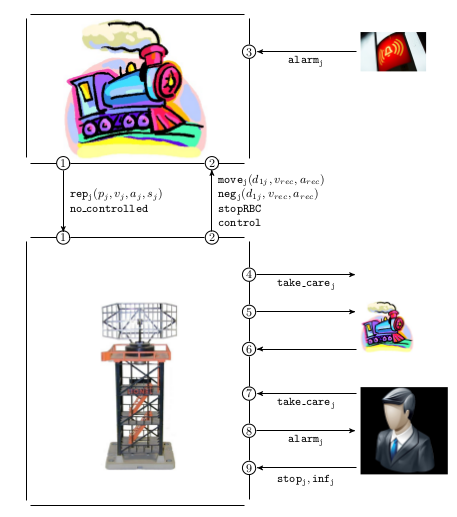
\includegraphics[width=.5\textwidth]{figures/ETCSModel.png}
  \caption{Main Actors in the ETCS.}
  \label{fig:model}
\end{center}
\sspace
\hrule
\end{figure}

1) According to the standards, the ETCS actors communicate in a distributed scenario that is characterized by the absence of a global time, thus, each player has its own clock. Moreover, there are two main safety issues related to time constraints. First, how often the train should report to RBC (position, speed, etc.) and how often the RBC has to send control messages to the train. We do not discuss this issue in the deliverable, since this decision is usually made when verifying the safety of a corresponding logic formula. In our model, this is modeled by discrete time instances when messages may be received/sent. The second aspect is related to the situation when, for some reason, exchange messages are lost. In order to deal with this situation we augment our model with timeout functions. If there is no input before the timeout expires then the player (RBC, a train under control, and/or the environment) has to make their own decision and for the safety issues usually it is the decision to stop the train. Therefore, in our model we synchronize the RBC and train by sending messages with relevant parameters such as the position, the maximum speed, the velocity, or the security point. 

2) Another portion of safety issues is related to situations when a train under control moves in an autonomous way: when the train should negotiate with RBC about the safety distance, when the train should be stopped, i.e., we have to check the functional aspects of the system. Some core points can be defined where an actor has different behaviors, and those points can be considered as states in the model. The conditions when an actor moves from one point (state) to another are usually related to some safety distances between trains, respecting alarm messages, etc. Transitions significantly depend on the values of continuous variables such as train position, speed, acceleration, etc. 

To solve these issues, we consider an ETFSM (Extended Timed Finite State Machine) as a formal model from which test cases for verifying the safety aspects of the developed implementations can be automatically generated. According to our model, there are three actors: a train under control, an RBC and the environment. The train under control has four states where it has different behavior. These states are depicted in Figure~\ref{fig:states}. 

\begin{figure*}[t]
\hrule
\sspace
\centering
  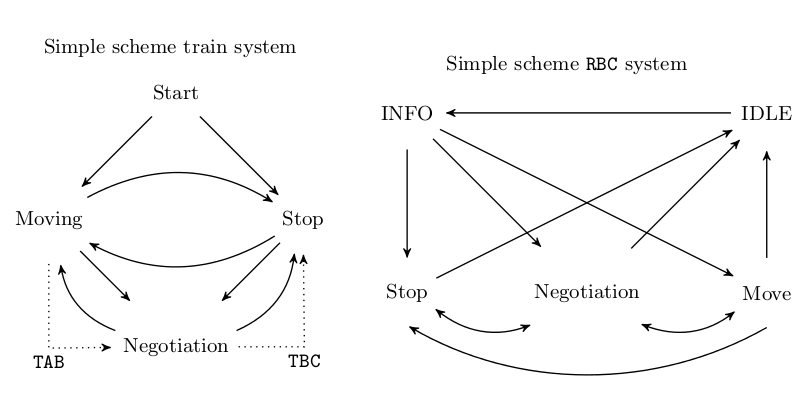
\includegraphics[width=.9\textwidth]{figures/ETCSStates.png}
  \caption{States of the train and \textit{RBC} models.}
  \label{fig:states}
\sspace
\hrule
\end{figure*}

\textbf{Start} The initial state is where the train gets a notification message informing that it is controlled by the given RBC. When getting this message the train reports the corresponding data to RBC and moves to another state (moving/stopping).

\textbf{Moving} At this state, the train can get different messages from RBC but almost any message should contain the safety distance according to the position of the previous train or possibly some obstacles reported to the RBC by the environment. If the train is in a safe position it continues moving in an autonomic way. However, if its position is closer to some dangerous point then the train should come to another state and start the negotiation with RBC.

\textbf{Negot} If the train crosses the dangerous point then the train should be immediately stopped. The safety point can be calculated by the RBC based on the data got from the previous train or on some data got from the environment.

\textbf{Stop} The train is not moving, and it waits for an input of RBC in order to start moving again. In our model, we have such an actor as the environment and as far as we know, the idea of modeling the ETCS environment never has been presented. The environment can send alarm messages to the RBC if something happens outside. We also model the train “red button” (accident, fire etc.) inside the train also by the environment and in this case, the train has to immediately report the situation to the RBC. The RBC states are almost the same as for the train but the RBC can get/send messages to/from the environment that usually is some automatic control (another RBC) or some manager in charge. Moreover, based on the collected information (from other RBC, from trains this RBC is in charge of, etc.) the RBC calculates the safety position for a given train and reports this position to the train. Below we present formula of how this safety position is calculated based on the ETCS requirements.

\paragraph{Modeling requirements}

In this subsection, we briefly describe the main requirements of the ETCS Level 3. In application Level 3 replaces the line-side signals as well as the trackside occupancy checking devices. The location of the train is determined by the trainside optometry and reported to the trackside radio block centre via the GSM-R radio transmission. In this configuration, train spacing is no longer controlled by the interlocking. However, the latter has to exchange information about the route setting with the RBC. In this level, the trains follow the moving block principle~\cite{platzer2009european}, i.e., the current speed and acceleration of a train are dynamically determined by a RBC tracking the train.  Trains are only allowed to move when the RBC grants them permission to do so. According to the set of requirements, in this model, we have the first the \textit{requirement R1} which is the critical point of \textit{Train$_{id}$} of interest (with respect to the previous train). This point is calculated by the RBC that controls the \textit{Train$_{id}$}  to avoid collisions. Figure 1 shows the states which are used in the representations of a train under control and an RBC that controls this train. 

Figure~\ref{fig:model} depicts the actors that are considered in the ETCS, i.e., should be presented in our model, and the exchange messages. The environment actor represents external inputs which may occur in the system, such as an alarm event or a call of an administrator that can interact with the RBC. Thus, the \textit{requirement R2} is also considered in the model.

The RBC analyzes the information obtained from the previous train and returns the critical distance d to the train. According to the rules, the safety distance \textit{requirement R3} is used in the model.

We say that a train at position p and with the critical point d is:

\begin{itemize}
\item In a \textit{safe} position if $(d - p) >= 4 SD$;
\item In a \textit{negotiation} position if $2 SD <=  (d - p) <=  4 SD$;
\item In a \textit{stop} position if $(d - p) < 2 SD$.
\end{itemize}

The developed model takes the above expressions into consideration: If the train is at the \textbf{Moving} state and it is in a \textit{safe} position then it can remain at this state having the speed and acceleration recommended by the RBC that controls the train. However, if the train progresses and the critical distance is not increased with the same speed, then the train will move to a negotiation position and enter the \textbf{Negotiation} state. Finally, if the train is at the \textbf{Negotiation} state and the critical distance does not increase then the train moves to a stop position and enters the \textbf{Stop} state where the train has zero speed. 

Also this model satisfies the \textit{requirement R4}.

To model this behavior the timeouts $TAB = 4 SD/Vmax$ and $TBC = 2 SD/Vmax$ are introduced in our model (where $Vmax$ is the maximum speed allowed for the train). If the train is at the \textbf{Moving} state and the train does not receive any message from the RBC then after $TAB$ time units it automatically moves to the \textbf{Negotiation} state, while if the train is at the \textbf{Negotiation} state and does not receive any input message from the RBC during TBC then the train moves to the \textbf{Stop} state.

\paragraph{Formal model}

We use the following functions when describing the set of transitions of the train and RBC models:

\begin{itemize}
\item The function $g(RBC)$ returns the critical point $d$ to the \textit{Train$_{id}$};
\item The function $f(Train_{id})$ returns the current position ($p$), speed ($v$) and acceleration ($a$) values and the next internal state of the \textit{Train$_{id}$} according to the values of the train sensors.
\end{itemize}

1) \textbf{The train}: An ETFSM that describes the internal behavior of the Train$_{id}$ has the following states. State \textbf{Start} is the initial state of the train. Any train at this state is not controlled by the RBC of our interest. Once the train is controlled it moves to the \textbf{Moving} state.

The RBC checks the position of the train at appropriate time units which usually are very close to each other. If the train crosses the Negotiation point then the train and the RBC start negotiating and the train moves to \textbf{Negotiation} state. The dot line $TAB$ denotes a timeout. If the train does not receive any input from the RBC during an appropriate time period (this is discussed above), then the train automatically moves to the \textbf{Negotiation} state.  The train is at this state if the train has crossed the Negotiation point but did not reach stop position yet; the RBC calculates a new critical position (point $d$).  If the train reaches Stop position then the train automatically should stop (moves to the \textbf{Stop} state). Otherwise, it continues moving and will go to the \textbf{Moving} state or stay at the \textbf{Negotiation} state depending on the value of $d$ and its current position. At the \textbf{Stop} state the train has the null speed. The train can come to this state if timeouts are triggered or the current position of the train is very close to the critical point, or the train has received an alarm message from inside the train (modeled as a part of the environment) or a \textit{stopRBC} message from the RBC.

2) \textbf{The RBC}: At the initial state \textbf{IDLE}, the RBC collects the information of all the trains which are controlled by this RBC and is waiting for the message \textit{take\_care} to control a train of interest.
 
When the message \textit{take\_care} is confirmed by the train then the RBC moves to the \textbf{Info} state. The \textbf{Info} is the state where the RBC waits for a message from the train that contains its position, speed and acceleration and its current internal state. 

The RBC sends the message \textit{control(k)} to the train in the \textbf{IDLE} state and when $k = j$ the train Train$_j$ is controlled by the RBC. Once getting the message \textit{control(j)} at the \textbf{Start} state the train replies with the message \textit{rep(p; v; a; state)} to the RBC. In fact, once controlled by RBC the train replies with this message to any input from the RBC. The message \textit{move(d; V$_{max}$; a$_{max}$)} sent to the train contains the critical point $d$ (with respect to the previous train or with respect to the next station etc.), the maximum speed $V_{max}$ and the maximum acceleration $a_{max}$ that the train can have. 

Depending on the position of the previous train and possibly other conditions, the critical point $d$ is calculated and according to its value the RBC moves to the \textbf{Stop} state, to the \textbf{Negotiation} state, or to the \textbf{Move} state. The \textbf{Stop} is a state where the RBC finds out that the train is stopped.

It could happen because the position of the train is close to the point $d$ (the train is in a Stop position) or if any external input alarm occurs. The \textbf{Negotiation} is a state that denotes an active exchange of messages between the train and the RBC since the train is not in a \textit{safe} position but did not reach a \textit{stop} position, i.e., the train is in a \textit{negotiation} position. The \textbf{Move} state denotes that the train is moving as autonomous as possible.

The RBC sends the message \textit{stopRBC} in order to stop the train. If the train receives this message at any state then the train moves to the \textbf{Stop} state. 

The message \textit{neg(d; $V_{max}$; $a_{max}$)} is sent to the train when the RBC knows that the train is at the \textbf{Negotiation} state. The environment can send the \textit{alarm} message to the RBC indicating that something is going wrong outside. 

Finally if the RBC gets this message then RBC sends the message \textit{stopRBC} in order to stop this train and enters the \textbf{Stop} state. There is a timeout $TAB$ from state \textbf{Moving} to the \textbf{Negotiation} state, where $TAB = 4 SD$ (four times exceeding the safety distance): 

\textit{If the train is in the \textbf{Moving} state and the train does not receive any input during $TAB$ time units, then the train automatically moves to \textbf{Negotiation} state.}

There also is a timeout $TBC$ from the \textbf{Negotiation} state to the \textbf{Stop} state, where $TBC = 3 SD$ (three times exceeding the safety distance) that means:

\textit{If the train is in the \textbf{Negotiation} state and the train does not receive any input after $TBC$ time units, then it automatically moves to the \textbf{Stop} state.}

\subsubsection{Using specification languages to describe the model}

\paragraph{Using XML and Java for model specification}

In order to assess the possibilities of the model to represent safety properties a prototype in XML-based language has been implemented that was then automatically translated into Java.

A simulator of an EFSM with timeouts has been developed: given a timed parameterized input sequence,  the simulator reproduces the corresponding sequence of outputs. In order to provide a clear representation of the model to the simulator, we depict all components using XML files. In each file, the main component is state and inside each state all its characteristics are presented. Among the possible things, there are transitions that start at this state, internal variables for each state, update functions for these variables and timeouts.  Once the XML file is properly defined, it is parsed, using JDOM - a Java library for XML parsing -  in order to create an internal representation of the ETFSM. During this phase, all the components are created internally to be used later for the simulation. After this phase is completed, the model is ready to be executed. The simulator itself is implemented in Java, with a different thread in charge of keeping time (issuing an alarm when a timeout has occurred). Also, each component is represented internally by a different object, for example transitions and timeouts are different object types with very distinct characteristics. 

Nevertheless, to perform model checking we have used different languages to specify the corresponding ETFSM. One of alternative can be the IF language which allows to efficiently specify train safety properties. 

\paragraph{Using IF for model specification}

IF is a language based on temporized machines, allowing the description of existing concepts into specification formalisms.  A real-time system described using IF language is composed of processes running in parallel and interacting asynchronously through shared variables and message exchanges via communication channels. The description of a system in IF consists in the definition of: data types, constants, shared variables, communication signals and processes. In Figure~\ref{fig:if:specification} we represent a short code of the ETCS system in this language.

\begin{figure}[t]
\hrule
\sspace
\centering
  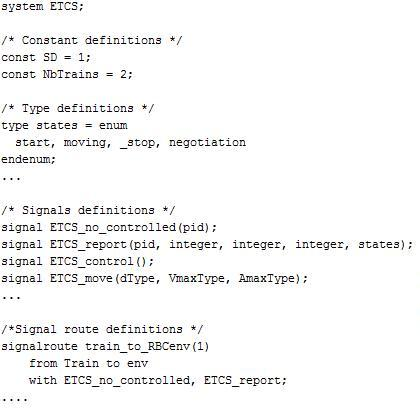
\includegraphics[width=.5\textwidth]{figures/test_generation.jpg}
  \caption{A sample code of the ETCS system specification in IF.}
  \label{fig:if:specification}
\sspace
\hrule
\end{figure}

\paragraph{Using SysML for model specification}

SysML (Systems Modeling Language) is a general-purpose graphical modeling language for systems engineering applications. It supports the specification, analysis, design, verification and validation of a broad range of systems and systems-of-systems. It is defined as an open source specification of a subset extension of the UML, i.e., SysML reuses seven of fourteen diagrams of UML and add two diagrams: requirement and parametric diagrams. It seeks to generalize UML for specifying complex systems that include non-software components such as information, processes, hardware, personnel and facilities.

In this project, we try to use SysML for model specifications. The SysML models are then validated by using SPIN model checker after translating them automatically into Promela.

\subsection{Model verification}\label{sec3}


\subsubsection{Deriving safety properties}\label{subsec3.1}


When performing the verification of the TEFSM model we considered the following safety properties.

\paragraph*{Property 1}

The train is in the \textbf{Moving} state, running at 100km per hour, with an acceleration of 10km per h² on a distance of 100km. Due to some external unexpected reasons, the train must stop as soon as possible. Therefore, an alarm from the environment is sent to the train. Automatically, the train should stop and provide a reporting message with its current parameters (state, position, etc.) to the RBC.

\paragraph*{Property 2}

In this case, the property is the capability of the ETCS system of taking over control if the driver appears to be going too fast.\footnote{This property represents the situation that caused the Spain train accident}  We consider the train in the \textbf{Start} state, receiving the message move with a certain speed and acceleration.

\paragraph*{Property 3}

A train is in the \textbf{Moving} state, running with a speed of 100 km per hour, with an acceleration of 10 km per h², situated somewhere at 10 km from the reference point. The safety distance ($SD$) between two ETCS trains is of 300 km. The train receives the signal move with the maximum speed of 105 km per hour and with an acceleration of 15 km per h² for the next 900 km.

\paragraph*{Property 4}

The property is related to transitions with time-outs. We consider a train in the \textbf{Moving} state, moving with a speed of 100 km per hour, with an acceleration of 10 km per h². The safety distance is of 300 km and the maximum speed allowed is $V_{max} = 105$ km per hour. 

The communication between the train and the RBC is lost, so the train should take an appropriate decision on the next state, after an appropriate period of time.
 
We further discuss different verification techniques that can be used to check the above properties based on the ETFSM.

\subsubsection{Proof technique}

A proof is a demonstration that if some fundamental statements (axioms) are assumed to be true, then some mathematical statement is necessarily true. As mentioned in the requirements document produced by WP2, as much as possible, formal proof would then be used to prove that the OpenETCS model never enter a Feared State, as long as the other subsystem (RBC, communication layer, etc.) fulfill their own safety properties (axiom describing the environment). Such theorem proving helps to increase our confidence on the specified model.  The proof techniques should be integrated in the selected tool chain. In order to use formal proof to verify if the SFM (Semi-formal model) and FFM (fully formal model) comply with the safety and function requirements (cf. R-WP2/D2.6-02-058), the properties to be proven have to be identified and described. There will be a set of axioms that will describe both functional and/or safety properties of the system. The choice of axioms describing functional and/or safety properties will be provided by safety analysis in an independent way from approaches used to specify, design, validate or verify. It must be noted that the model obtained from the Subsystem Requirements Specification should be verified in this manner at a first stage.

\subsubsection{Model checking}

Model checking is an automatic technique for verifying finite-state reactive systems. Using such techniques one could automatically check if the model specifies most of the requirements of the system, such as the important safety properties described in Task 4.4. Similar to proof techniques, in order to use model checking to verify if the SFM (Semi-formal model) and FFM (fully formal model) comply with the safety and function requirements (cf. RWP2 /D2.6-02-058), the properties to be proven have to be identified and described. To implement the use model checking, it is mandatory to specify the model using finite-state reactive systems, and they should also provide an intuitive way to express the properties to be model checked. The language for describing a formal model for which corresponding model checkers exist should be selected and the set of critical requirements to be verified need to be clearly identified. The proposed model checking techniques should be supported in the selected tool chain. As mentioned above, we are using XML-based and IF-based specification to perform the model checking of train safety properties.

\subsubsection{Simulation}

When using model checkers the criteria for the model to be safe is that all the safety properties should be checked. The latter is impossible, since the number of safety properties is infinite and thus, only some of them can be checked through the above step.

For this reason, as a complementary approach, testing is commonly used. If the corresponding model respects safety requirements, i.e., only expected outputs are produced to applied input sequences, to some extent, there is a confidence that the models is safe. In order to derive ‘good’ tests a formal model should be involved. It is known that only the FSM model where each input is followed by a corresponding output allows automatic deriving finite tests with the guaranteed fault coverage where the races between inputs and outputs can be easily avoided.  Many authors for deriving finite tests with the guaranteed fault coverage turn their model to some kind of an FSM (see, e.g.,~\cite{springintveld2001testing,zymc11,Gromov2009}). 

As for simulation, the artifacts should provide means to execute the model.  The simulator must be automatically generated, so that, when run against test scenarios (inputs/outputs for the model), we may conclude whether the model follows the specification or not. In particular, it is important to define test scenarios for the safety critical properties. Since, the developmentwithin openETCS has to the goal to reach the CENELEC EN 50128 SIL 4 standard, it is highly recommended (cf. SIL 4) that the simulation needs to cover all states, transitions, data-flow, and paths in the model. It would also be desirable to include graphical representation of the simulation/model and also provide a report of the visited components as specified by CENELEC EN 50128 SIL 4. CENELEC EN 50128 SIL4 also advocates to perform tracing. Being able to trace the requirements that are met during a simulation is also advisable to allow simple requirement coverage.

\subsubsection{Other Methods}

Reviews, Inspections, static analysis and walkthroughs, mostly manual techniques, are also to be considered for the verification of models. 

\subsection{Existing software tools for model verification}\label{sec4}

\subsubsection{SPIN model checker}

SPIN (Simple Promela INterpreter)~\cite{Holzmann97} is an open-source software too1, written in C, for simulating and verifying concurrent systems. The communications, via message channels, between concurrent processes of system can be synchronous, i.e., rendezvous, or asynchronous, .i.e., buffered. Models of systems to be analyzed are described by Promela (PROcess MEta LAnguage). In simulation mode, the model is executed step-by-step to familiarize with the behaviors of system. In verification mode, the model is exhaustively explored in order to show that it satisfies some critical properties, e.g., deadlock-free, violated assertions, or general correctness requirements given in Linear Temporal Logic formulas. In this mode, SPIN generates a C program that constructs an implementation of the model-checking algorithm for the given model. The program is then compiled and run to get the result.

As SPIN is proven to be efficient model checker we further plan to try a model checking approach using Promela specification. For this purpose, we will derive a Promela specification from of the ETFSM and perform the model checking of safety properties. Such safety properties will be specified as assertions, and corresponding violations will provide the counter-examples if the model will be invalid.

\subsubsection{Using Java Pathfinder model checker}

Java Pathfinder~\cite{JPF} (JPF) is a system to verify executable Java bytecode programs. The core of JPF is a Java Virtual Machine that is also implemented in Java. JPF executes normal Java bytecode programs and can store, match and restore program states. Its primary application has been Model checking of concurrent programs, to find defects such as data races and deadlocks. 

As in this project, the XML-specification of the train system is automatically converted into Java code we also consider to use this model checker in the future. In this case, safety properties will be specified as Java assertions and will be added to the corresponding Java implementation. 

\subsection{Testing European Train Control System}\label{sec5}

\subsubsection{Adaptive scenario} 

In this section, we present the notion of testing and discuss a testing scenario for our model. We assume that the RBC and the train are tested separately, i.e., when testing the train software the RBC is replaced by a tester that sends inputs to the train and checks whether the produced outputs are expected. Moreover, we consider adaptive testing, i.e., a test case is represented as an acyclic ETFSM~\cite{Petrenko2011,offutt1989coupling} where only one timed input is defined at each intermediate state. We start at the initial state and apply an input defined at the state to an IUT. Based on the produced output the FSM R that represents a test case will move to another prescribed state where another input can be specified and exactly this input will be applied at the next step.  If the observed trace is a trace of the specification ETFSM then we say that the IUT passed a test case. Otherwise, the IUT fails the test case, i.e., the IUT does not conform to the given specification. We illustrate our approach using the following testing scenario (Figure~\ref{testing:scenario}):

\begin{figure}[t!]
\hrule
\sspace

\begin{minipage}{0.3\hsize}
\centering
\textbf{Step 1}\\

	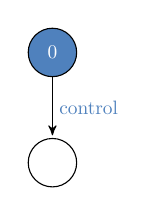
\begin{tikzpicture}[>=stealth',shorten >=1pt,auto,node distance=2cm,scale=0.7, every node/.style={scale=0.7}]
	  \node[state, fill=hblue, text=white] (A)      {$0$};
	  \node[state]         (B) [below of=A]  {};
	 
	 
	  \path[->] 
		(A) edge  node [hblue] {control} (B)
	;
	\end{tikzpicture}

\end{minipage}
\begin{minipage}{0.7\hsize}

\textbf{Step 2}\\

	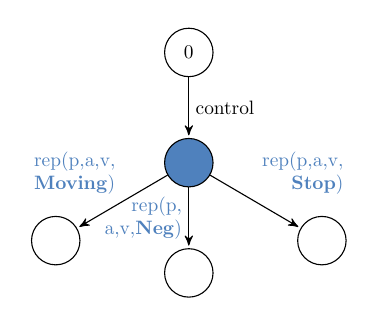
\begin{tikzpicture}[>=stealth',shorten >=1pt,auto,node distance=2cm,scale=0.7, every node/.style={scale=0.7}]
	  \node[state] (A)      {$0$};
	  \node[state, fill=hblue]         (B) [below of=A]  {};
	  \node[state]         (C) [below left of=B,xshift=-1cm]  {};
	  \node[state]         (D) [below of=B]  {};
	  \node[state]         (E) [below right of=B,xshift=1cm]  {};
	 
	 
	  \path[->] 
		(A) edge  node {control} (B)
		(B) edge  node [hblue,align=left, above left] {rep(p,a,v,\\\textbf{Moving})} (C)
		(B) edge  node [hblue, align=right, left ] {rep(p,\\ a,v,\textbf{Neg})} (D)
		(B) edge  node [hblue, align=right] {rep(p,a,v,\\\textbf{Stop})} (E)
	;
	\end{tikzpicture}

\end{minipage}

%\begin{minipage}{1\hsize}


\centering
	\textbf{Step 3}\\

	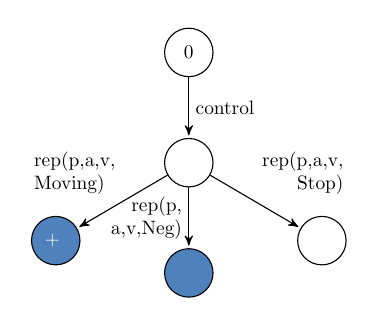
\begin{tikzpicture}[>=stealth',shorten >=1pt,auto,node distance=2cm,scale=0.7, every node/.style={scale=0.7}]
	  \node[state] (A)      {$0$};
	  \node[state]         (B) [below of=A]  {};
	  \node[state, fill=hblue, text=white]         (C) [below left of=B,xshift=-1cm,align=center]  {\TAB + \TBC};
	  \node[state, fill=hblue, text=white]         (D) [below of=B]  {\TBC};
	  \node[state]         (E) [below right of=B,xshift=1cm]  {};
	 
	 
	  \path[->] 
		(A) edge  node {control} (B)
		(B) edge  node [align=left, above left] {rep(p,a,v,\\Moving)} (C)
		(B) edge  node [align=right, left ] {rep(p,\\ a,v,Neg)} (D)
		(B) edge  node [align=right] {rep(p,a,v,\\Stop)} (E)
	;
	\end{tikzpicture}

\textbf{Step 4}\\

	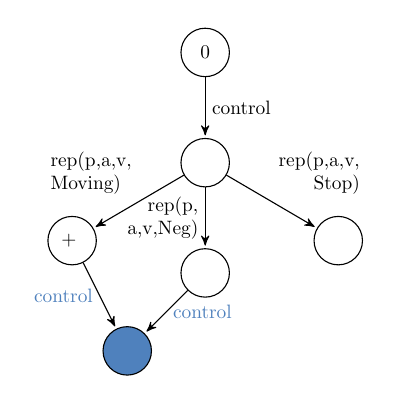
\begin{tikzpicture}[>=stealth',shorten >=1pt,auto,node distance=2cm,scale=0.7, every node/.style={scale=0.7}]
	  \node[state] (A)      {$0$};
	  \node[state]         (B) [below of=A]  {};
	  \node[state]         (C) [below left of=B,xshift=-1cm,align=center]  {\TAB + \TBC};
	  \node[state]         (D) [below of=B]  {\TBC};
	  \node[state]         (E) [below right of=B,xshift=1cm]  {};
	  \node[state, fill=hblue]		   (F) [below left of=D] {};
	 
	 
	  \path[->] 
		(A) edge  node {control} (B)
		(B) edge  node [align=left, above left] {rep(p,a,v,\\Moving)} (C)
		(B) edge  node [align=right, left ] {rep(p,\\ a,v,Neg)} (D)
		(B) edge  node [align=right] {rep(p,a,v,\\Stop)} (E)
		(C) edge  node [hblue, left] {control} (F)
		(D) edge  node [hblue, right] {control} (F)
	;
	\end{tikzpicture}


%\end{minipage} 
%\begin{minipage}{0.3\hsize}

\centering
		\textbf{Step 5}

	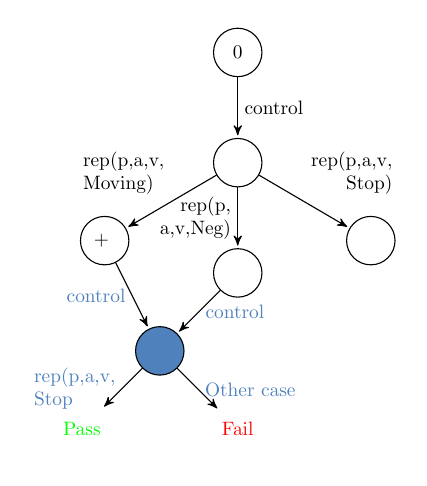
\begin{tikzpicture}[>=stealth',shorten >=1pt,auto,node distance=2cm,scale=0.7, every node/.style={scale=0.7}]
	  \node[state] (A)      {$0$};
	  \node[state]         (B) [below of=A]  {};
	  \node[state]         (C) [below left of=B,xshift=-1cm,align=center]  {\TAB + \TBC};
	  \node[state]         (D) [below of=B]  {\TBC};
	  \node[state]         (E) [below right of=B,xshift=1cm]  {};
	  \node[state, fill=hblue]		   (F) [below left of=D] {};
	 \node[state]		   (G) [below left of=F, white, text=green] {Pass};
	 \node[state]		   (H) [below right of=F, white, text=red] {Fail};
	 
	  \path[->] 
		(A) edge  node {control} (B)
		(B) edge  node [align=left, above left] {rep(p,a,v,\\Moving)} (C)
		(B) edge  node [align=right, left ] {rep(p,\\ a,v,Neg)} (D)
		(B) edge  node [align=right] {rep(p,a,v,\\Stop)} (E)
		(C) edge  node [hblue, left] {control} (F)
		(D) edge  node [hblue, right] {control} (F)
		(F) edge  node [hblue, left, align=left] {rep(p,a,v,\\Stop} (G)
		(F) edge  node [hblue, right] {Other case} (H)
	;
	\end{tikzpicture}

%\end{minipage}

\caption{Testing scenario.\label{testing:scenario}}
\sspace
\hrule
\end{figure}


\textit{If there is no signal from RBC (lost messages) for an appropriate period of time then a train must stop itself.}

In Figure~\ref{testing:scenario} are represented the following five steps:

\begin{enumerate}
\item The tester (simulating the RBC functioning) starts with sending the message control to the train. The 0 value in the initial state means that the RBC does not wait anything to send this message.
\item Depending on the internal state of the train, the tester moves to different states. In order to simplify the example let us consider that the train always answers this message.
\item At these states the tester waits for the appropriate number of time units $TAB + TBC$ or $TBC$ when there are no messages sent to the train.
\item Then the tester checks the state of the train by sending the control message again.
 If the train is in the \textbf{Stop} state then the tester returns \textit{Pass}, otherwise it returns \textit{Fail}. Finally, having the train at the \textbf{Stop} state the tester forces it to move with the maximal permissible speed and acceleration and returns the critical distance $d$.
\end{enumerate}
 
In the same way, other testing scenarios for checking safety properties may be considered. For example, we can derive a test case that checks whether a train stops when being close to the critical point $d$, a test case that checks whether a train changes the Moving state when crossing the critical point $d$, a test case that checks whether a train speed (acceleration) does not exceed the permissible maximum, etc. Finally, it is worth mentioning that when we are testing whether a train stops when reaching a critical point or whether the train respects RBC requirements about its speed and acceleration we must use continuous variables.

\subsubsection{Test generation based on IF representation}

In this Section we present how to automatically extract a set of tests from the specification. To do this, the behavior of the train process is described in the IF language. We have identified a set of basic requirements and we can describe them as properties in IF.  Based on these properties, the validation and verification of the formal specification are carried out using the IF toolset TestGen-IF which automatically generate a set of adaptive tests.

We present a short overview of the result of applying this tool in a requirement related to Property 1 (Section~\ref{subsec3.1}). The set of test objectives associated to this scenario, noted as OBJ(1) is formally described in Figure~\ref{set:of:tests}.

\begin{figure}[t]
\hrule
\sspace

\begin{lstlisting}
#Test-case for the train in the Moving state
?ETCS_control{}!ETCS_report{{Train}0,10,100,10,start}
?ETCS_alarm_to_train{}!ETCS_report{{Train}0,10,
	100,10,moving}
?ETCS_control{} !ETCS_report{{Train}0,10,0,0,_stop}
#Test-case for the train in the Negotiation state
?ETCS_control{}!ETCS_report{{Train}0,10,100,10,start}
?ETCS_move{900,105,15}!ETCS_report{{Train}0,10,100,
	10,moving}
?ETCS_alarm_to_train{}!ETCS_report{{Train}0,10,100,
	10,negotiation}
?ETCS_control{}!ETCS_report{{Train}0,10,0,0,_stop}
\end{lstlisting}
\caption{Set of test using TestGen IF tool.\label{set:of:tests}}
\sspace
\hrule

\end{figure}


Let us note that, according to the system specification, the property OBJ(1) is correct in any of the states of the train model. Therefore, at any state, the train should stop when receiving an external alarm input.

Different test scenarios are performed with respect to safety properties discussed in Section~\ref{subsec3.1}. As a future work we plan to verify the fault coverage of these tests by executing Java simulator against corresponding traces.


\subsection{Results/Conclusions}

In this deliverable, we have provided a formal model for the requirements of the European Train Control System using finite state machines augmented with continuous variables (train position, speed, acceleration) and time constraints. The model is a very close representation of the system specification provided by the standard.

We have discussed different model checking techniques to verify safety properties for corresponding ETFSM representing the ETCS. To efficiently perform such model checking we use different specification languages, namely, XML and IF languages.
%
We have proposed a technique of the ETCS adaptive testing w.r.t. test scenarios written as train safety properties. 

As a future work, we plan to use different model checkers and perform experiments with the model being derived. We plan to use SPIN and for this purpose we will specify the TEFSM in the SysML language that will be further translated into Promela. Meanwhile, we plan to use the JPF model checker to efficiently utilize the Java train simulator that has been developed during the first part of the project.

\newpage

\section{TWT GmbH Science \& Innovation: Verification of Procedures of Subset
026-5}

This sections reports on the modeling of the procedures described in Subset 026, Chapter 5---that is, the behavioral part of the ETCS. The goal of the activity is to validate the specification and to support the modeling using SCADE and the verification of SCADE models on a higher\footnote{in comparison to SCADE models} level of abstraction.

The activity is described in the Verification and Validation Plan (see Sect.~6.1.2.5). In short, we provide feedback regarding ambiguities, inconsistencies and errors in the current ETCS standard based on our formalization of the specification using mathematical modeling languages.

\paragraph{Object of verification}

The object of verification is Subset 026-5 of the specification. We formally model parts of the specification and use the resulting model to validate the specification. This design step has been described in D2.3 (see Sect.~4.4).

\paragraph{Available specification}

The specification is described in Subset 026-5. It describes procedures of ETCS entities (i.e., required reactions on events and received messages), thereby focusing on required change in status and mode of entities considered.


\paragraph{Detailed verification plan}

\subparagraph{Goals} 

The goal is to model the the procedures described in Subset 026-5, thereby focusing on modeling the \textit{system behavior}---that is, the control flow of the on-board unit and the interplay with its environment (e.g., the driver and the RBC). The model is then used to validate the specification.

\subparagraph{Method/Approach}

As a formal model, we use \textit{colored Petri nets} (CPNs)~\cite{CPN-book}, an extension of classical Petri nets~\cite{PNbook} with data, time, and hierarchy. CPNs are well-established and have been proven successful in numerous industrial projects. They have a formal semantics and with CPN Tools~\cite{Westergaard2013apn}, there exists an open source tool for modeling CPNs. Moreover, CPN Tools also comes with a simulation tool and a model checker, thereby enabling formal analysis of CPN models. 

We focus on modeling the \textit{system behavior}---that is, the control flow of the on-board unit and the interplay with its environment (e.g., the driver and the RBC). Figure~\ref{fig:Top} depicts the CPN representing the highest level of abstraction. It shows the decomposition of the overall system into the on-board unit and its environment: the driver, the RBC, the RIU, the STM, and the GSM module. Each component is modeled as a subpage (i.e., a component). Graphically, a subpage is depicted as a rectangle with a double-lined frame. Furthermore, the model shows through which message channels and shared variables the on-board unit is connected to its environment. A channel or shared variable is modeled by a place which is graphically represented as an elipse. As an example, the driver (i.e., subpage \texttt{Driver}) may send a message to the on-board unit (i.e., subpage \texttt{On-board Unit}) via the place \texttt{msg from driver}, and receives messages sent by the on-board unit via the place \texttt{msg to driver}.

\begin{figure}[tb]
	\centering
		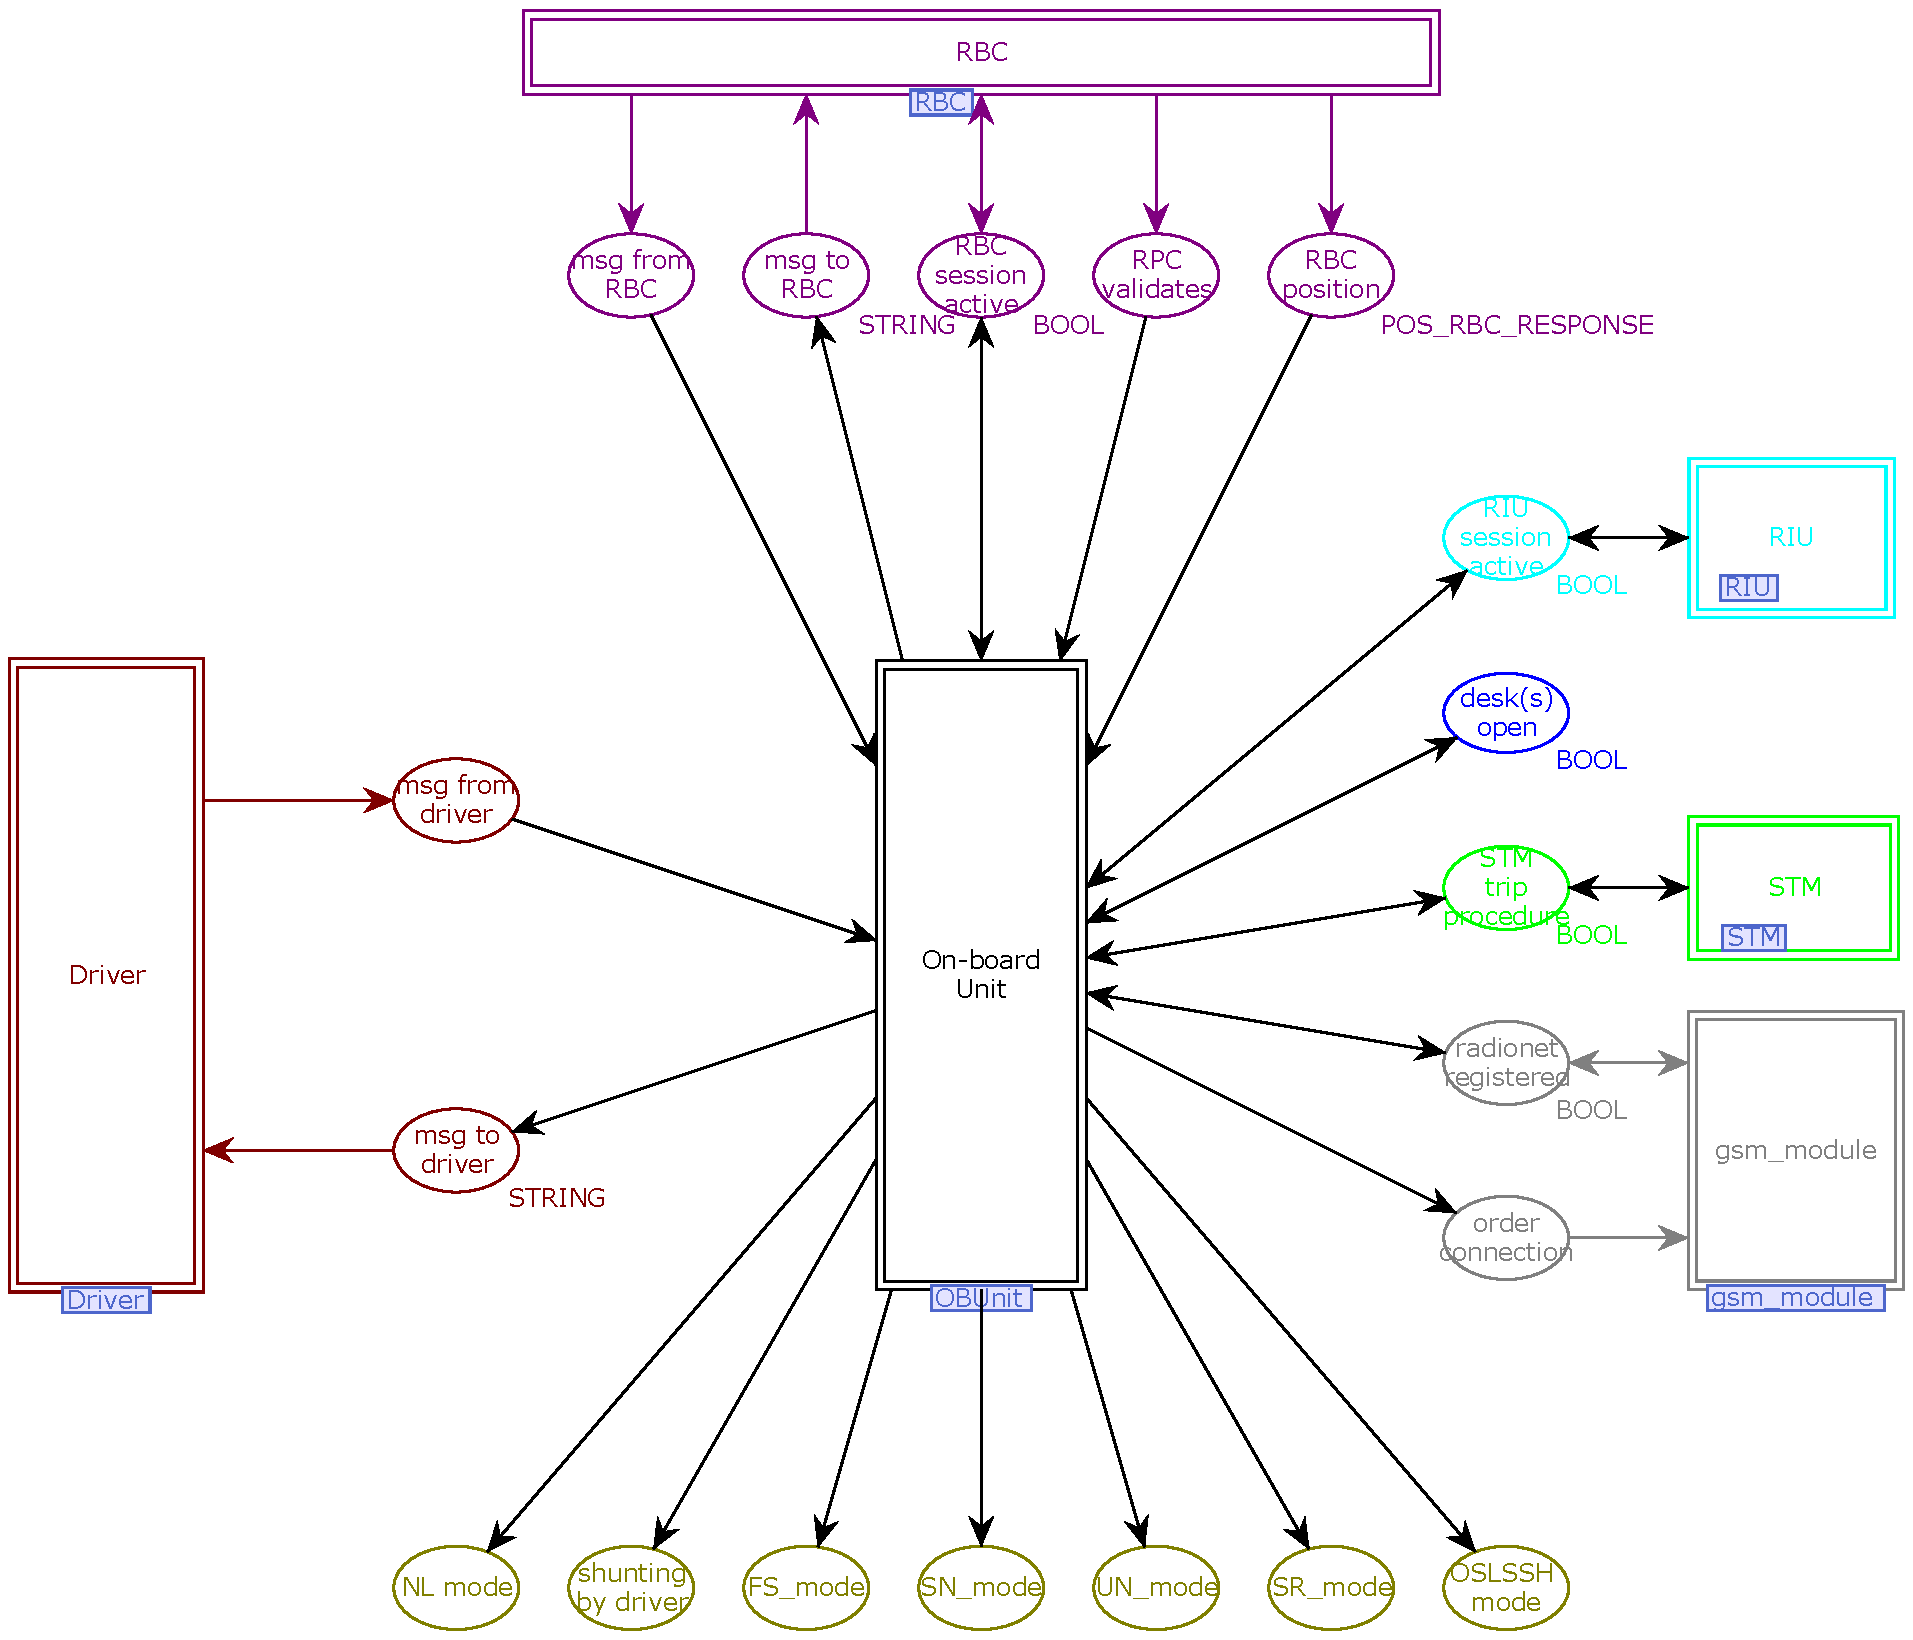
\includegraphics[width=0.9\textwidth]{figures/Top.pdf}
	\caption{Top level model}
	\label{fig:Top}
\end{figure}

Zooming in subpage \texttt{On-board Unit} yields the CPN model in Fig.~\ref{fig:OBUnit}. This CPN model has two subpages: Subpage \texttt{Start} models the states S0 and S1 of the specification (i.e., Subset 026-5.4) and subpage \texttt{Rest} the remaining states. At this level of abstraction, we see on the left hand side seven places (green frame). Each such place models (a part) of the state of the on-board unit, for example, the mode and the train running number. The current model has 689 places, 173 transitions and 1,227 arcs.

\begin{figure}[tb]
	\centering
		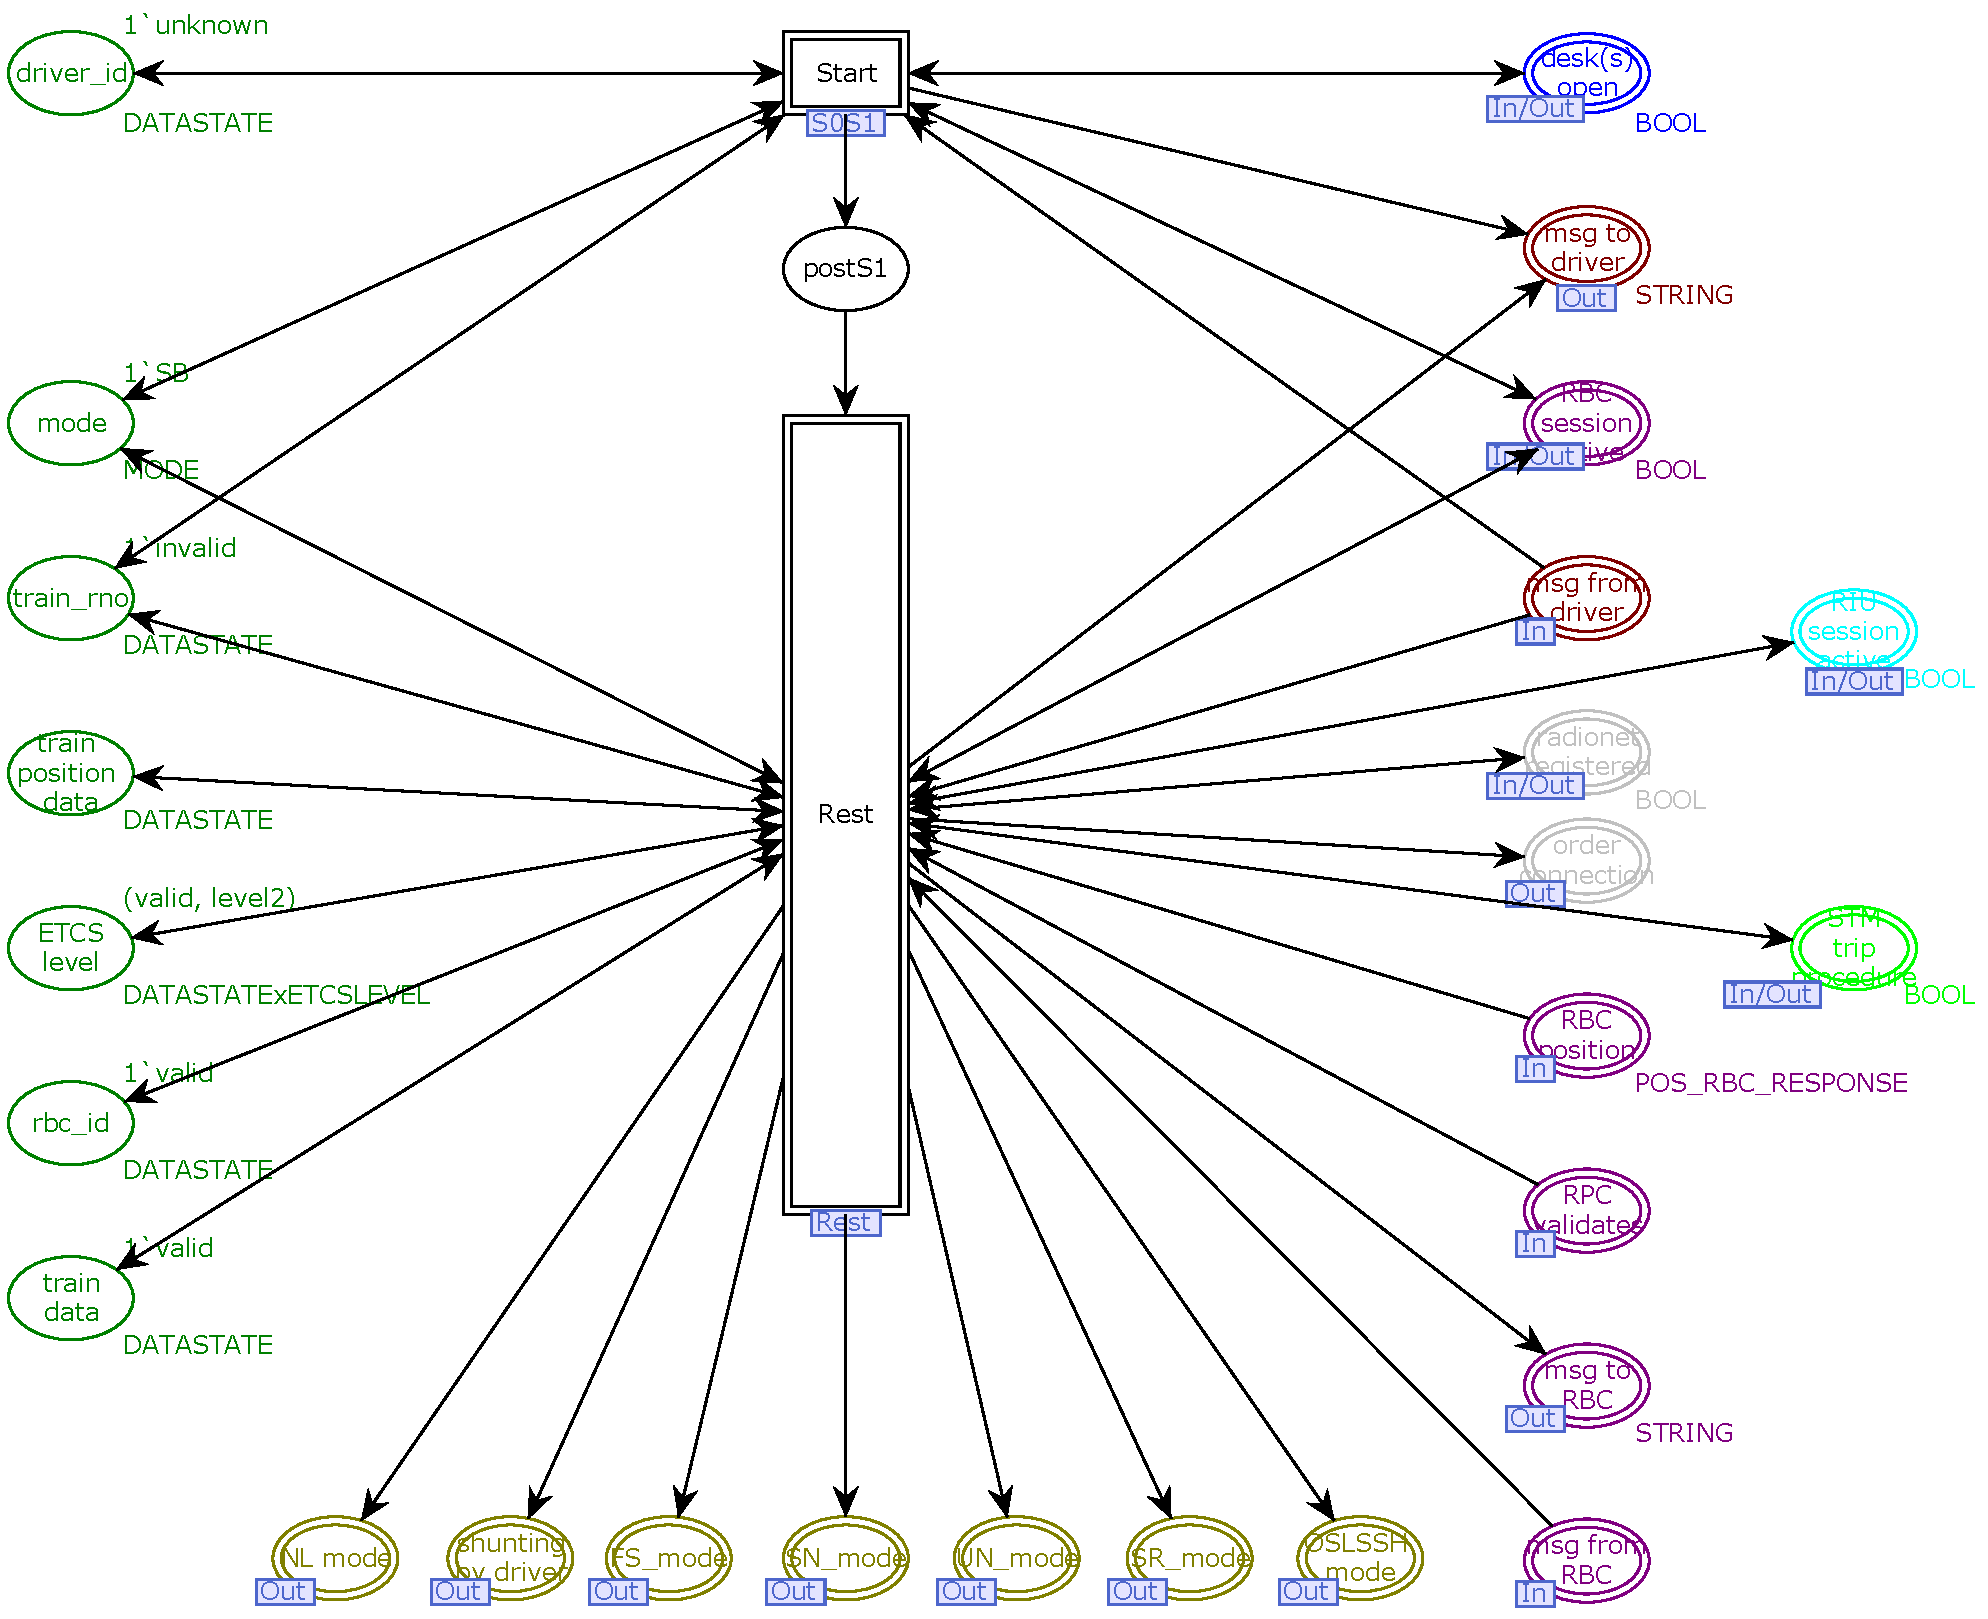
\includegraphics[width=0.9\textwidth]{figures/OBUnit.pdf}
	\caption{CPN model of the on-board unit}
	\label{fig:OBUnit}
\end{figure}

Having a more detailed look at Fig.~\ref{fig:OBUnit}, we observe that our model does not represent all variables of the on-board unit as given in the specification and also partially abstracts from data. We abstract from those details, because the model is tailored to formalize the \textit{control flow} of the on-board unit and, in particular, the \textit{communication behavior} with its environment. As a benefit, this abstraction reduces the complexity of the model and improves its understandability. Additional details, such as data and precise message values, can be added in a refinement step.

The modeled procedures have been manually modeled using CPN Tools. Thereby, each element in the model has been reviewed against the respective requirement, as given in the specification. To improve the confidence in the model, in a second step, a person other than the modeler checked the model against the specification. In addition, we used the simulator to check whether the modeled behavior of the CPN matched the intended behavior.

So far, the primary goal of modeling has been to validate the specification. During the modeling we discovered 36 inconsistencies, ambiguities and gaps in the specification which we reported in~\cite{specfindings}. 


\subparagraph{Means}

The input for our approach is the specification described in Subset 026-5. Our output is a CPN model and a report describing inconsistencies, ambiguities and gaps in the Subset 026-5.


\paragraph{Results}

\subparagraph{Summary}

We have modeled the following five procedures of Subset 026-5 as CPN:
\begin{itemize}
	\item Start of Mission (Subset 026-5.4)
	\item End of Mission (Subset 026-5.5)
	\item Shunting Initiated by Driver (Subset 026-5.6)
	\item Override (Subset 026-5.8)
	\item Train Trip (Subset 026-5.11)
\end{itemize}
During the modeling we discovered 36 inconsistencies, ambiguities and gaps in the specification which we reported in~\cite{specfindings}. Our CPN models the system behavior---that is, the interplay between the different entities of the ETCS---and partially abstract from data. Therefore, we complement the work on SysML modeling, where the focus is on the connectivity of components and the data types.
 
\subparagraph{Conclusions/Lessons learned}
 
The numerous specification findings illustrate the need for validating the specification. CPNs are well-suited to model the behavioral aspects described in Subset 026-5. The size of the model clearly indicates the complexity of the procedures, even at the current level of abstraction. Therefore, we expect that applying formal verification on the resulting CPNs will not be feasible due to state-space explosion.

\paragraph{Future Activities}


We shall continue our work by completing the model, contributing to the modeling of (parts of) Subset 026-5 using SCADE, and verifying the SCADE model. In addition, we are planning to exploit synergies by collaborating with the project partner LAAS who advocate the Petri net model checker TINA~\cite{BerthomieuV2006}. In addition, we are working with the project partners from Braunschweig University of Technology on generating test cases from the CPN model.


\paragraph{Modeling the Subset 026-5}

We plan to model the remaining parts of Subset 026-5, thereby reporting possible additional findings in the specification. The goal is to have a CPN modeling all procedures that are described in Subset 026-5. We also want to compare our model with the (corresponding part of the) ERTMSFormalSpec model~\cite{ertms}.


\paragraph{SCADE Modeling}

As the ETCS will be modeled using SCADE, we shall contribute to this modeling process. To use the experience that we gained from modeling Subset 026-05 with CPN Tools, we want to contribute to the SCADE modeling of (parts of) the Subset 026-5. The SCADE design flow starts with modeling all components and their interplay using SysML block diagrams (with the tool SCADE Designer). The resulting SysML diagrams provide a functional and an architectural view. They are similar to the CPN model in Fig.~\ref{fig:Top}. In a second step, the behavior of each block has to be fully modeled on the system level using SCADE Suite. Currently, SCADE does not support state machine models on the level of SysML. Our CPN model provides this level of abstraction and will, therefore, be useful for the SCADE modeling.


\subparagraph{Verification of the SCADE Model}

Another task concerns the verification of the resulting SCADE model. Recently, researchers reported on complexity problems already for medium-sized SCADE models that restrict the verification using the SCADE prover~\cite{HuhnM2014scp,DaskayaHM2011fmics}. Given the complexity of the ETCS, we assume that we will face similar challenges. To alleviate those complexity problems, we aim to apply the following three techniques:

\begin{description}
	\item[Abstraction:] We will apply abstraction techniques on the SCADE model to prove safety properties on a higher level of abstraction whenever possible. On the one hand, we can apply SCADE contracts to restrict the domain of the input values. This technique is known as environment abstraction. On the other hand, we can transform the SCADE model into a model of higher abstraction, thereby using different formalisms such as timed automata, transition systems and Petri nets. (As SCADE has a formal semantics such transformations are possible, but may take considerable effort.) We can then use verification tools that are dedicated to the properties of interest and the chosen formalism. We see the chance that our CPN model can be used for this task, too. For example, Uppaal~\cite{BehrmannDLHPYH2006} can analyze timed automata, the Spin model checker~\cite{Holzmann97} and NuSMV~\cite{CimattiCGGPRST2002} can analyze transition systems, and TINA~\cite{BerthomieuV2006}, LoLA~\cite{Wolf2007}, and CPN Tools~\cite{Westergaard2013apn} are tools for analyzing (different variants of) Petri nets.
	%
	\item[Compositional Reasoning:] Another approach is to prove properties for individual components and deduce from it the correctness of a property concerning the entire ETCS. Here we think that we can, in particular, combine our model with the MoRC model~\cite{braunstein_MorC_2013} and apply compositional reasoning.
	%
	\item[Correctness by Design:] The two previous approaches support \textit{correctness by verification}; that is, first the model is designed and in the next step it is verified. A different methodology is \textit{correctness by design}. The idea is to model on a higher level of abstraction and to prove that certain safety properties hold. Then the model is iteratively refined. Each refinement step has to guarantee that all properties that hold for the more abstract level also hold in the refined model. The challenge is to find property-preserving refinement rules or a refinement relation between an abstract model and a refined model that preserves the desired properties and to verify that this relation holds. The results can be applied to validate the SCADE model and the specification.
\end{description}





\newpage

\section{UniBremen}


\newcommand{\tbi}[1]{$<$\textit{#1}$>$}

% Starts a new line nearly everywhere
\newcommand{\nl}{\mbox{}\\}
\newcommand{\nlskip}[1]{\mbox{}\\[#1]}

%
%Comments
\newcommand{\cmmnt}[1]{\framebox{#1}}
\newcommand{\bgcmmnt}[1]{\nl\framebox{\parbox{.95\textwidth}{#1}}\nl[2mm]}
%\renewcommand{\bgcmmnt}[1]{}
%

\newcommand{\eod}{\nl\rule{.95\textwidth}{1pt}\nl\textit{End of Document}}


\section{University of Bremen: Verification of the  Management of the Radio
Communication}
\label{sec:ubremen}
This section reports the verification activity of SCADE-MoRC. The goal
of this activity is, first, to establish the compliance of the SCADE
model to the SRS description via testing. Secondly, we want to track
the ambiguities within the specification. Finally we want to
demonstrate the efficiency of model based testing using the RT-tester
tool for system integration testing.

The activity is described in the Verification and Validation Plan
section {\em 6.1.2.7 System Integration Testing (Uni Bremen/DLR)} \cite{D4.1_2013}.
In short, we develop a test model from the specification, generate tests and use
the code generated from SCADE to perform software-in-loop testing.
The test model and the SCADE model used to generate code have been
done independently to each other. 

\paragraph{Object of verification}
 Management of radio communication (MoRC) ERTMS function baseline 3.


The system under test (e.g. the verification object) is the C code
generated from a SCADE model and described here
\url{https://github.com/openETCS/model-evaluation/tree/master/model/SCADE_Siemens/Subset_026_Chapt_3.5_ManagementOfRadioCommunication/Generated_C_Code}.
It describes the Management of the radio communication at the software
phase.




\paragraph{Available specification}

The specification is described in the
Subset-026 chapter 3.5. It
describes the communication protocol between the EVC and the RBC or
balises. In particular, how the EVC initiates and terminates a
communication.



\paragraph{Detailed verification plan}

\subparagraph{Goals}

To achieve what has been defined previously a test model in SysML has
been developed. The description of this verification artifact may be
found here \url{https://github.com/openETCS/model-evaluation/blob/master/model/EA-SysML/new_version/doc/ea_sysml_report.pdf}

Our main goal is to verify the SCADE model by test simulation. The
tests are produced by a model of the Subset-026 chapter 3.5 described as a
state machine.

\subparagraph{Method/Approach}

\begin{figure}
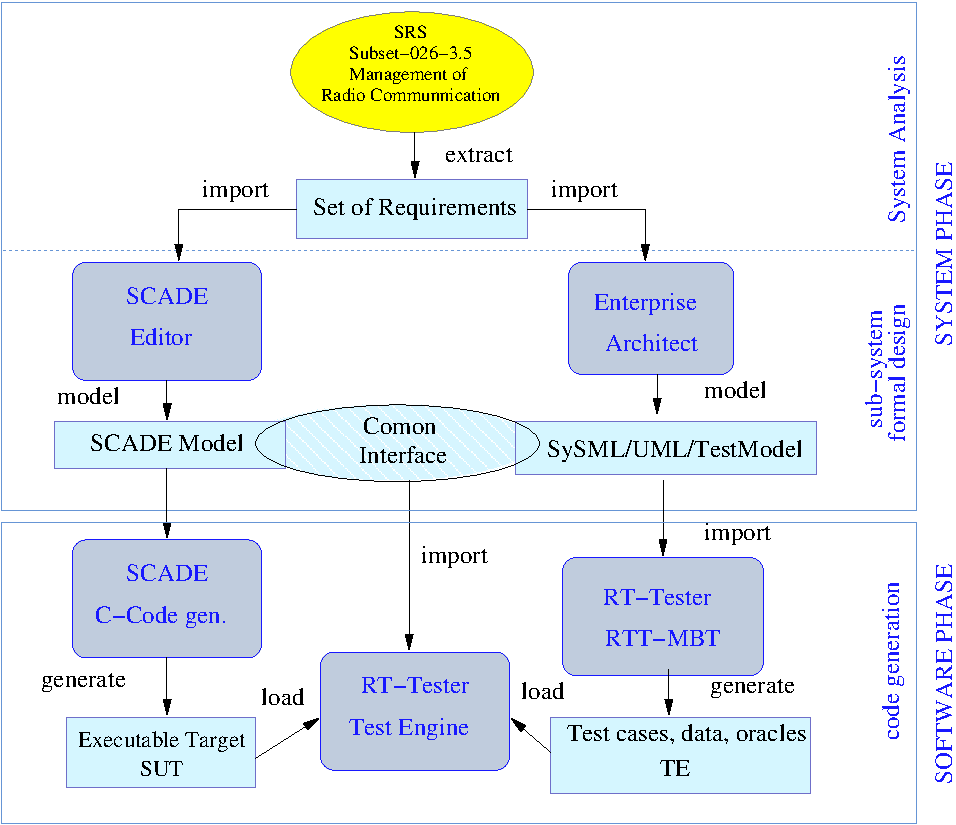
\includegraphics[width=\textwidth]{schema/framework}
\caption{\label{fig:method}SCADE/RT-Tester methodology}
\end{figure}

Figure \ref{fig:method} depicts our methodology. From the SRS
specification, two models are designed: one SCADE model that will
be then  used to produce C code and one SysML model for generating
tests.

Our test model contains the behavioral representation of the MoRC, the
set of requirements of the chapter 3.5, and the link between the behavior
and the requirement.  Most of the requirements may be represented as
single transition or state in the test model state
machine. Nevertheless, some of the requirements may be only modeled as
a path of the state machine, we choose to represent those as LTL
formula, added as constraints of the test model. For example the
\verb+REQ-3.5.3.10+ describes the steps needed for the establishment of
the radio communication order by the RBC. This requirement explicits a
particular path of the test model, thus this path should exists in our
test model. To ensure that this particular test will be generated a LTL
formula has been added (See \cite{braunstein_MorC_2013} for more
details).

\begin{description}
\item[REQ-3.5.3.10] "If the establishment of a communication session is
initiated by the RBC, it shall be performed according to the following steps
..."
\vspace{-1em}
\begin{verbatim}
Finally (MessageIn == INIT_SESSION_TRACK && setUp == 1 -> 
Next (MessageOut == SESSION_ESTABLISHED && radioComSession == ESTABLISHED)
\end{verbatim}
\end{description}

We need then to link the system under test and the test model. Since
the two models are elaborated independently, we need to ensure that
the tests generated may be handled by the code generated by SCADE and
conversely we need to read the output of the C code back to the test
generator to compare the values with our oracles. This is achieve by
defining a common interface that the two models should respect. The
inputs drive the tests and the outputs are the observational points to
state if a test pass or fail. Hence, the two models should respect the
same interface.

After the modeling phase, starts the test generation phase.
Two strategies have been used for the tests generation. First, we
generate a set of test following the common behavioral coverage
strategies ensuring the following coverage :
\begin{itemize}
\item  Basic control state coverage (BCS): All state locations are covered.
\item  Transition coverage (TC): All transition of the statecharts are covered.
\item  Modified condition/decision coverage (MC/DC): Modified condition/decision coverage.
\item  Hierarchic transition coverage (HITR): High-level transition of
  nested statecharts are covered.
\item  Basic Control states Pair coverage(BCPAIRS): For concurrent state
  machines pair states of two different state machines. 
\end{itemize}

More detailled explaination on the coverage may be found here \cite{huang_test_2013}.

We then apply a requirement coverage strategy to
generate tests that covers all the requirements. 
As each requirement
is linked to an artifact of the test model, part of the test cases
are generated as subset of the coverage mention above. In addition,
test cases from the LTL are also provided.


Finally the test engines run the SUT with the stimuli from the test
model. In parallel, it runs the test oracles that states if the test
pass or fail.

\subparagraph{Means}

The Artifacts are produced as follow:
\begin{itemize}
\item C code comes from SCADE model.
\item Test model is a SysML model designed with Enterprise Architect.
\item Test cases, tests data and test oracles are generated with RT-tester.
\item Executable code compile with gcc.
\item Code run within the RT-Tester engine.
\end{itemize}

SCADE is EN 50128 qualified at SIL 3/4, RT-tester is also certifiable
T3 as shown in \cite{peleska_efficient_2012}.

\subsection{Results}

\begin{table}[htbp]
\centering
\begin{tabular}{lr}\toprule
  Coverage strategies & \# tests generated  \\\midrule
  BCS & 14 \\
  TC & 40 \\
  MC/DC & 79 \\
  BCPAIRS & 33\\
  HITR & 12 \\
  LTL & 2 \\ \midrule
  Total Tests& 180\\\bottomrule
\end{tabular}

\vspace{1em}
%\raggedleft Total Requirements cover 40
\caption{\label{tbl:test_summary} Test cases generation summary}
\end{table}

Table \ref{tbl:test_summary} resumes the set of automatically
generated tests.
The set of tests cover 40 of the requirements from the chapter 3.5.


The simulation result of the C code is not yet finished and for the
moment, all test failed. The main reason was that the two
models did not share the same starting condition.
Hence, we  need to refined our test model to be able to handle SCADE
modeling style correctly and be able to have interesting result.



\paragraph{Summary}

What we have done:
\begin{enumerate}
\item Created a test model in SysML.
\item Generated test cases.
\item Ran SCADE model against test procedure produces by RT-tester.
\end{enumerate}
 
 The next step:
 \begin{enumerate}
 \item Refined test model
 \item Analyze the result of the test procedure.
 \item Coordinate DLR/SIEMENS/Uni Bremen interfaces.
 \item Run the test on the DLR lab.
 \end{enumerate}

\paragraph{Conclusions/Lessons learned}

Our first attempt to simulate the tests was not a success. All tests
except the one covering the initial states failed. Our two models
have, at least, the same initial state.
From  our first investigation, we could see that one chapter of
the specification is not self-contained. This leads to different
interpretation in the modeling and thus some non equivalent behaviors.

Moreover some missing information in the specification leads to 
 constraints in test model. It affects the test generation by
providing some non realistic test cases. Some variable behavior that
were not mentioned in the specification are considered as free and may have any
possible value in their definition range. This can be solved by adding
information into the test model. 

More precisely, the test model is composed with a system under test
and a test environment. In our first model the test environment is
empty, meaning that all inputs of the SUT are free. The test
enviroment may be described (and constrainted) by statecharts or
LTL formula that restricts the behaviors of the inputs. The test
generator should then find  test suites that realize the given
coverage and that respect the constraints given in the test environment.



\paragraph{Future Activities}
\subparagraph{Refine the test model}
\begin{enumerate}
\item Analyze the test results of the SCADE C code
\item Enumerates specification ambiguitites: where the two parties did
  not undestand the specification in the same way.
\item Refine the test model by adding a better test environment with
  the help of domain experts
\end{enumerate}
\subparagraph{New activities}
We will also provide the ceiling speed monitoring function to enrich
the test model and apply new model based testing approach.

%\bibliographystyle{plain}
%\bibliography{biblio}



\newpage

\section{University of Rostock }

%\documentclass{article}
%\usepackage{hyperref}
%\usepackage[utf8]{inputenc}
%\usepackage{graphicx}
%\usepackage{booktabs}
%\graphicspath{{schema/}}
%\title{Performance Estimation of the Speed and Distance Monitoring}
%
%\author{Alexander Nitsch \and Benjamin Beichler}
%\date{\today}
%
%\newcommand{\tbi}[1]{$<$\textit{#1}$>$}
%
%% Starts a new line nearly everywhere
%\newcommand{\nl}{\mbox{}\\}
%\newcommand{\nlskip}[1]{\mbox{}\\[#1]}
%
%%
%%Comments
%\newcommand{\cmmnt}[1]{\framebox{#1}}
%\newcommand{\bgcmmnt}[1]{\nl\framebox{\parbox{.95\textwidth}{#1}}\nl[2mm]}
%%\renewcommand{\bgcmmnt}[1]{}
%%
%
%\newcommand{\eod}{\nl\rule{.95\textwidth}{1pt}\nl\textit{End of Document}}
%
%\begin{document}
%\maketitle
%\begin{abstract}
%  This document reports the verification activities of the University of Rostock. SystemC (performance analysis), executable models: SysML modelling and code generation, Scade modeling and code generation.
%\end{abstract}


\subsection{Verification of the Speed and Distance Monitoring}

This section reports the verification activities of the \emph{Speed and Distance Monitoring} with model based simulation and virtual prototyping. The first activity pursues the goal of formalizing the specification in the form of an executable model. This model provides a performance estimation at an early stage of system level design and adduces evidence what hardware resources will be needed for the future OBU. Secondly, finding and reporting of unclarities, inconsistencies, incompleteness and errors while implementing the specification by using tools of the openETCS toolchain (Papyrus/SysML, SCADE). Furthermore, we are developing a method of SystemC code generation from abstract and domain specific SysML models. Finally we want to demonstrate the efficiency of model based simulation after transformation from SysML to SystemC models.

The activity is described in the Verification and Validation Plan
section {\em 5.3.10 Verification with Model-Based Simulation} \cite{D4.1_2013}
To sum up, we develop application models from the specification of the \emph{Speed and Distance Monitoring}, generate test scenarios and use the inherent simulation environment of SystemC to do performance and scheduling analysis.

\paragraph{Object of verification}  Speed and Distance Monitoring ERTMS function baseline 3.
The system under test is the implemented SystemC code which is described here: \url{https://github.com/openETCS/model-evaluation/tree/master/model/SystemC_TWT_URO/3.13_Speed_and_distance_monitoring}. It describes the Speed and Distance Monitoring at the Software phase.
\nl

\begin{figure}[h]
\centering
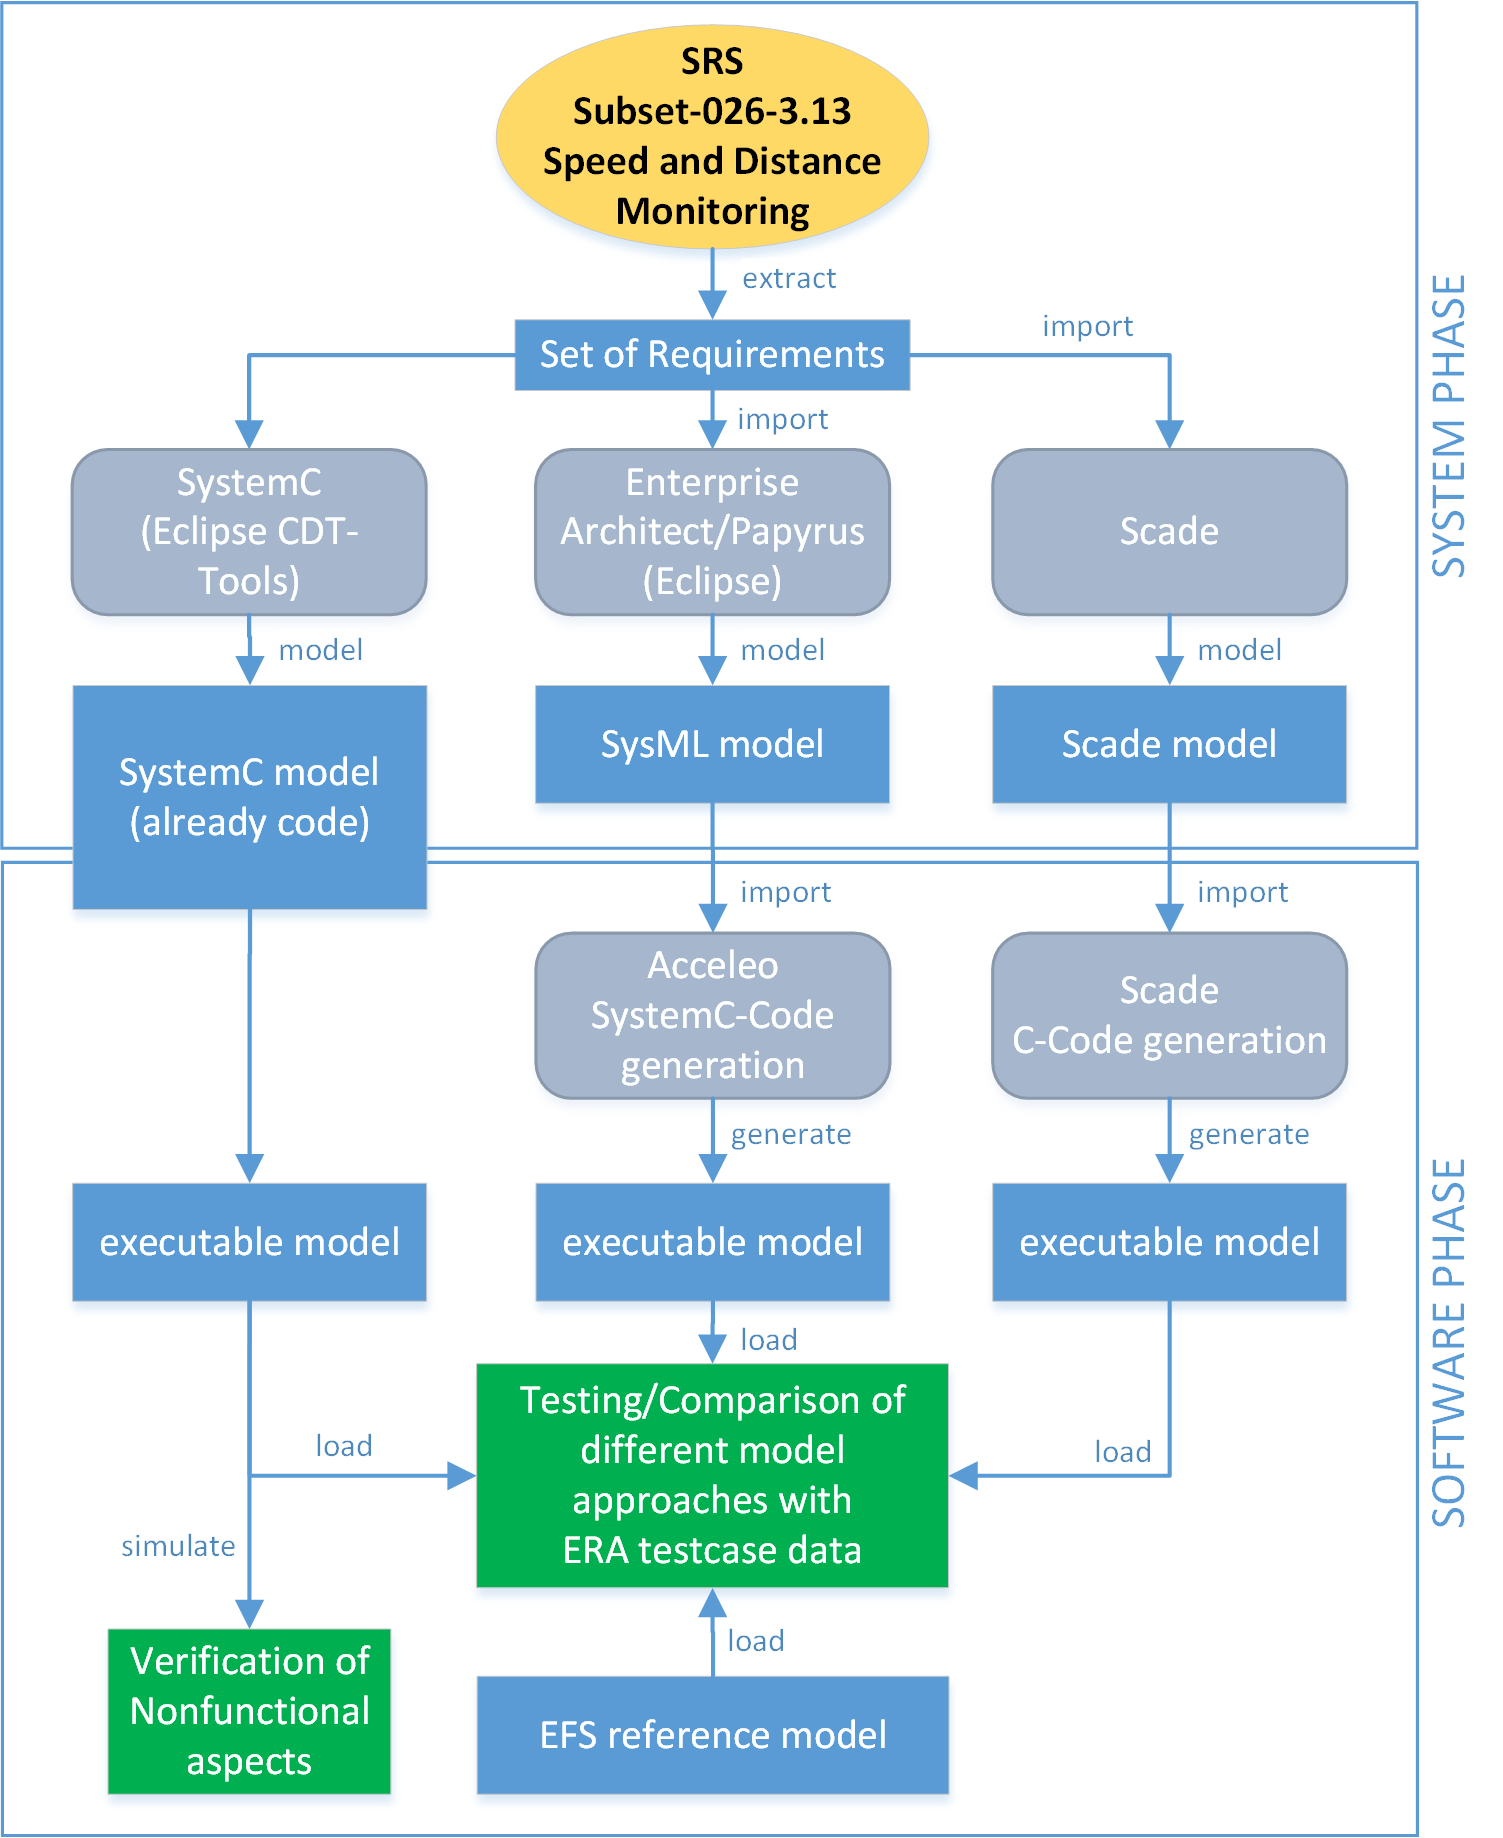
\includegraphics[width=.80\textwidth]{schema/UniRostockApproach.png}
\vspace{4mm}
\caption{University of Rostock VnV Approach}
\label{fig:University of Rostock VnV Approach} 
\end{figure}

\paragraph{Available specification}

The specification is described in the
SUBSET-026 Chapter 3.13 \cite{unisig_subset-026_2012}. It describes the realization of both TI and DMI commands by calculating several modules with inputs form train side, track side an odometry. The University of Rostock focuses on the calculation of parts, which are used for safety critical cases using emergency brakes. This especially includes the EBD (emergency brake deceleration) curves.

\paragraph{Detailed verification plan}

\subparagraph{Goals}

On the one hand we are testing extra-functional aspects such as performance and scheduling analyses to give evidence which hardware system is sufficient to meet the system requirements. We want to discover which hardware resources (e.g. number of processors) will be needed for the OBU. This is important to avoid excessive delays to ensure adequate response times in critical situations. Therefore the University of Rostock will do model based simulation using the inherent simulation environment of SystemC.

On the other hand we use the existing SystemC model to check against a reference model, such as EFS braking curve model. Furthermore we use different tools and means to build additional system models for comparison and verifying behavior.

\subparagraph{Method/Approach}

Figure \ref{fig:University of Rostock VnV Approach} depicts our methodology. Three models will be created from the SRS
specification: one SystemC model that is directly implemented into executable code (finished), one SysML model that will be used to produce SystemC code to be executable (not finished) and one SCADE model that will be used to produce C code (not finished). For model verification we use test cases and data provided by WP4 and use the ERA excel datasheet as reference implementation. The created test models will contain behavioral representation of the \emph{Speed and Distance Monitoring} such as state machines, activity diagrams and sequence diagrams. There will be a link to the specification requirements to meet the needs of traceability in terms of verification activities.


\subparagraph{Means}

The Artifacts are produced as follow:
\begin{itemize}
\item SystemC code which is directly implemented.
\item One Test model is the SystemC model. It's code will be generated/transformed by Acceleo from abstract SysML models designed with Enterprise Architect and/or Papyrus.
\item C code is produced by Scade using Scade System.
\item Executable code is compiled with GNU-C-Compiler \texttt{gcc}.
\item Reference model delivered by ERTMS Formal Specs.
\item Testdata and testcases are provided by ERTMS Formal Specs using the ERA excel data sheet.
\end{itemize}

\subsection{Results}

Verification of extra-functional aspects is successfully done for the first iteration of application models. The provided results consist of recommendations on how hardware resources shall be allocated to the future OBU. The modeling activities are still in progress.

\subparagraph{Summary}

What we have done:
\begin{enumerate}
\item Created an executable model in SystemC.
\item Ran simulations on single, dual and multi core virtual prototypes.
\item Architecture SysML model of the \emph{Speed and Distance Monitoring}.
\item Architecture Scade model of the \emph{Speed and Distance Monitoring}.
\item Defined a reduced set of parameters for calculating braking Curves especially EBD curves.
\end{enumerate}
 
 The next step:
 \begin{enumerate}
 \item Finishing model activities on SysML and Scade.
 \item Developing a model transformation/code generation from SysML models.
 \item Defining an exchanges interfaces between different model approaches.
 \item Run the tests.
 \end{enumerate}
\subparagraph{Conclusions/Lessons learned}
From the first results, we see that SysML is a very powerful graphical modeling language but to perform code generation it is necessary to have restrictions to it. We will have a domain specific SysML profile to get reliable results from code generation.  


\paragraph{Future Activities}
Simulink as a modeling tool is in our interest because there is a bridge to Scade. Simulink provides code generation for hardware description languages such as VHDL. That enables new hardware test scenarios.

\newpage

\section{Systerel}

Three approaches of VnV  on formal models have been experimented and are presented in this section:

\begin{enumerate}
\item VnV on classical B  model that cover software design level, in the objective to provide an open-source approach;
\item VnV on Event-B model that cover system level and support safety analysis;
\item VnV on Scade model that cover software design level.
\end{enumerate}

Classical B and Scade model specify the same example of Subset 026 "§5.9 Procedure on-Sight", Event-B model specifies the "Mangement of Radio communication" function.

\documentclass{article}
\usepackage[utf8]{inputenc}
\usepackage{amsmath}
\usepackage{url}
\usepackage{amsfonts}
\usepackage{graphicx}

\title{Verification and validation of B~models}
\author{Benoît~Lucet\\Systerel}
\date{\today}

\begin{document}

\maketitle

\begin{abstract}
This document describes the verification and validation processes applicable to B~models. It supports B as a promising method in the context of openETCS, given the maturity and level of rigor associated with it.\\
After an introductory section where we discuss the subject of validation, section \ref{sec:processes} presents the different verification processes and discusses their advantages and drawbacks, while section \ref{sec:tools} presents the tools available to perform such verification. Finally, appendix \ref{app:osproc} presents the application of the verification process to an existing B example: the procedure on-sight.
\end{abstract}

\newpage

\tableofcontents

\newpage

\section{Introduction}
\label{sec:intro}
A B~model is a textual and formal specification covering the functional behaviour of a safety critical software. It is usually written based on a high-level specification (informal or formal specification, for example SysML or a natural language). It is gradually refined, starting at the top with an abstract notation and ending at the bottom with sequential instructions --- which are then auomatically translated in a target language such as C or Ada.\\
Thus, we define three objects of verification and validation: the specification, the B~model and the generated source code.\\

Validation consists of:
\begin{itemize}
\item guaranteeing the functional adequacy between the specification and the model (this can be achieved, for example, through review and proofreading),
\item building a test environment around the generated source code and test it.
\end{itemize}
Hence, this document will mainly focus on verification, i.e.\ the methods and tools required to assure that B~method is a consistent way of producing critical software.

\section{Verification processes applicable to a B~model}
\label{sec:processes}
In this section, we demonstrate the suitability of the B~method towards the problematics encountered in the openETCS project by introducing the different verification processes applicable to a B~model.\\
Each of the verification process is presented and its contributions to the system security and consistency are discussed.

\subsection{Type checking}
Static type checking (TC) is a basic form of program verification that ensures type safety of the model. It is the first verification --- after lexical and syntactic analysis --- to be performed on a B~model, thus allowing an early detection of problems. It is also a pre-requisite for the higher-level verifications. \\
Strong typing ensures a consistent use of data and is essential to writing correct formulae (predicates or expressions).\\

The type checking process consists of two main activities: data typing and type verification.\\
{\itshape Data typing} is the activity of assigning a type to newly-encountered data in a predicate or a substitution\footnote{In B, a substitution is comparable to a set of instructions that modify variables. For more information, see \cite{bbook}.}. It is based on an inference mechanism, which is able to deduce the type of a newly-encountered variable from the type of the other variables intervening in the predicate or the substitution, and specific inference rules.\\
On the other hand, {\itshape type verification} is the activity of verifying typing rules between already-typed variables. These rules are specific to their applying predicates, expressions or substitutions.
% In B, the base types consist of integers, booleans, strings, abstract sets and enumerated sets.\\
% The construction of more complex types is achieved through the powerset operator $\mathbb{P}$ and the cartesian product $\times$.

\subsection{B0-check}
The B0 verification has the specific purpose of checking the respect of the rules that the B~model has to conform to in order to generate the translation to C or ADA. These rules are called implementability rules and must be respected in order for the translation to process properly. They also ensure that the resulting code is executable and respects a set of properties.

\subsection{Well-definedness}
An expression is well-defined (WD) if its associated value or interpretation exists and is unique, thus avoiding ambiguity.\\
Examples of ill-defined formulae include division by zero, function application to an argument out of the domain, function application of a relation etc.\\

Well-definedness checking is thus an extra verification that helps strenghten the model.

\subsection{Model checking}
Model checking is a static semantic check that searches for invariant or assertion violations and deadlock states.\\
This type of verification animates the model, modifying the current state of the machine, starting from the initialization. Operation calls are simulated and modify the internal state which is then checked for various properties. Most of the time, an invariant or assertion violation is looked for.\\

This verification process, as opposed to the ones previously introduced, considers the semantics of the model and aims at verifying properties dynamically. However, it has its limitations:
\begin{itemize}
\item unability to run through all of the states and transitions,
\item difficulty to deal with infinite sets.
\end{itemize}
This means that potential erroneous states can be missed, and that this verification process is not sufficient to ensure {\itshape correctness}, though satisfying as an additional verification tool.

\subsection{Constraint-based checking}

Constraint-based checking (CBC) is the process of finding a given valid state, for which an operation call leads to an erroneous state. This is done by constraint solving instead of --- as seen for model checking --- running through states from the initialization.\\
This technique will usually provide more counter-examples than model-checking, because it ignores the initialization constraints and can thus reach a wider range of states.

\subsection{Formal proof}
A proof obligation is a mathematical lemma generated by the proof obligation generator (POG). It corresponds to a consistency property of the model, that has to be demonstrated.
A fully-proved model is said to be {\itshape correct}, in the sense that every property (invariant, assertion) expressed is proved to hold for every state of the program. If a proof obligation is not provable, it means that the B~model is inconsistent and must be corrected. In fact, the goal of any B development is to obtain a proved model.\\
In contrast to model-checking, formal proof does not require to make assumptions about the size of the system (number of transitions). It is reliable and powerful, but it needs to be taken into account that:
\begin{itemize}
\item some proofs can be very difficult to solve,
\item the model needs to be written as to make it the simplest to prove, which demands experience and skill.
\end{itemize}
A proved model will always meet the safety and security qualifications~; however that doesn't mean it will behave in regards to the specification! This is the domain of validation, as discussed in the introduction.

\section{Tools for verification}
\label{sec:tools}

\subsection{Existing tools}
In this section, we present the existing tools suitable for the verification processes defined in section \ref{sec:processes}.

\subsubsection{Atelier~B}
\label{subsec:atelierb}
Atelier B\footnote{See \url{http://www.atelierb.eu/en}} is the main development tool associated with the B~method and is produced and distributed by ClearSy. It provides most of the needed tools.

\paragraph{B~compiler}~\\
The B~compiler performs syntax analysis, type checking, identifier scope resolution and B0-checking. It is part of Atelier~B as an open source tool.

\paragraph{Proof obligation generator}~\\
Atelier~B's POG is currently the only known fully operational POG for B, and is free of charge --- although proprietary software, which means closed-source. ClearSy is currently working on a new proof obligation generator~; whether it will be open source or not is to be determined.

\paragraph{Prover, proof assistant, user-defined rules}~\\
Atelier~B provides a free of charge --- although not open source --- prover which discharges proof obligations. Depending on the complexity of the model, a varying proportion of the proof obligations is discharged automatically.\\
For the remaining proof obligations, Atelier~B provides an interactive proof assistant allowing the user to guide the prover in discharging the PO. The user may define theories (or rules) which have in turn to be proved. The user-defined rules are organized in a database. 

\paragraph{Atelier~B translators}~\\
Translators are an essential component of the industrial success of B. The translators take the B0 implementations as input and produce a target source code, typically Ada or C/C++, ready to be compiled or integrated in an environment.\\
ClearSy provides an open source translator, but it does not reach the T3 level of qualification\footnote{For additional information on qualification, see subsection \ref{subsec:qualif} or the CENELEC norm.}.

\subsubsection{ProB}
\label{subsec:prob}
ProB is an animator and model checker for B~models distributed under the EPL license (open source) and mainly developed by Formal Mind\footnote{See \url{http://www.formalmind.com}}.\\
It performs model checking as well as constraint-based checking and searches for a range of errors, with customizable search options and various graphical views. ProB also handles automatic coverage reports generation.\\
ProB is a mature tool and is being used by several industrials such as Siemens and Alstom. This makes it a precious tool for the verification processes described above.

\subsection{Tool qualification}
\label{subsec:qualif}
Atelier~B has been used for many years to develop railway critical software. It is, for this exact reason, {\itshape qualified} by the main actors of the railway domain: SNCF, RATP, Alstom, Siemens etc.\\

The CENELEC norm defines qualification levels for verification tools. Annex A 5 of the norm specifies several verification techniques and for each of them, a recommendation level (mandatory, higly recommended, recommended). Below are listed the different techniques and measures along with their recommendation levels:
\begin{enumerate}
\item Formal Proof (HR)
\item Static Analysis (HR)
\item Dynamic Analysis and Testing (HR)
\item Metrics (R)
\item Traceability (M)
\item Software Error Effect Analysis (HR)
\item Test Coverage for code (HR)
\item Functional/ Black-box Testing (M)
\item Performance testing (HR)
\item Interface testing (HR)
\end{enumerate}

Table \ref{tab:cenelec} shows, for each of the verification processes presented in \ref{sec:processes} (specification and source code were added), the corresponding item in the CENELEC norm annex table.

\begin{table}[h!]
\begin{center}
\begin{tabular}{ l c c c c c c c }
~ & spec & TC & B0C & MC & CBC & proof & source code \\
\hline
A 5.1 & ~ & ~ & ~ & ~ & ~ & \checkmark & ~ \\
\hline
A 5.2 & ~ & \checkmark & \checkmark & ~ & \checkmark & ~ & ~ \\
\hline
A 5.3 & ~ & ~ & ~ & \checkmark & ~ & ~ & ~ \\
\hline
A 5.4 & ~ & ~ & ~ & ~ & ~ & ~ & ~ \\
\hline
A 5.5 & \checkmark & ~ & ~ & ~ & ~ & ~ & ~ \\
\hline
A 5.6 & ~ & ~ & ~ & ~ & ~ & ~ & ~ \\
\hline
A 5.7 & ~ & ~ & ~ & ~ & ~ & ~ & ~ \\
\hline
A 5.8 & ~ & ~ & ~ & ~ & ~ & ~ & \checkmark \\
\hline
A 5.9 & ~ & ~ & ~ & ~ & ~ & ~ & ~ \\
\hline
A 5.10 & ~ & ~ & ~ & ~ & ~ & ~ & ~ \\
\hline
\end{tabular}
\end{center}
\caption{Correspondence between CENELEC norm recommendations and the presented verification processes}
\label{tab:cenelec}
\end{table}

\subsection{Conclusion on tools}
Table \ref{tab:comparison} summarizes the presentation of the tools in subsections \ref{subsec:atelierb} and \ref{subsec:prob}.\\
Atelier~B and ProB are both mature tools that have proved their worth. They are the core tools for validation processes of B~models. However, key components of Atelier~B are not open source and this issue is not completely compensated by ProB's model checking and CBC.\\
An ongoing research project named BWare\footnote{See \url{http://bware.lri.fr/index.php/BWare_project}} and conducted by ClearSy, Inria, LRI and others aims at providing a framework from proof obligation generation to proof discharge by the means of SMT solvers. This promising project started in September 2012 and is funded for a period of four years. It opens perspectives for the near future in terms of open source B~model verification.

\begin{table}[h!]
\begin{center}
\begin{tabular}{l c c c c c}
~ & TC & B0 & model check. & CBC & proof \\
\hline
B~Compiler & \checkmark & \checkmark & ~ & ~ & ~ \\
\hline
POG and provers & ~ & ~ & ~ & ~ & \checkmark \\ 
\hline
ProB & ~ & ~ & \checkmark & \checkmark & ~ \\
\hline
\end{tabular}
\end{center}
\caption{Comparison of the tools available for B verification processes}
\label{tab:comparison}
\end{table}

\section{Conclusion}
The B~method, along with its verification processes and tools, meets the goals and activities of the openETCS project in terms of quality, rigor, safety and credibility.\\
There is yet to develop open-source POG and build a framework for proving, but this is compensated by the fact that work on the subject is ongoing, and ProB is an effective tool for verification.

\newpage

\appendix
\section{Application: Procedure On-Sight}
\label{app:osproc}
The Procedure On-Sight, as described in {\itshape System Requirements Specification, Chapter 5}, has been modelled in B\footnote{The model is available at \url{github.com/openETCS/validation/tree/master/VnVUserStories/VnVUserStorySysterel/02-DAS2V/c-ClassicalBModel/ProcedureOnSight}.} to show the feasibility of the task and the credibility of the method. This appendix briefly presents the model, then applies the verification processes to this example.

\subsection{Presentation of the B~model}
As shown in figure \ref{fig:procos}, the model is split into three main processing modules, one of which corresponds to the actual on-sight procedure,
and the two others being used as data conditioning:
\begin{itemize}
\item \verb+os_mode_level+: determines the ETCS level and the mode. Contains the on-sight procedure algorithm,
\item \verb+os_consist+: checks data consistency, provides adaptation to the current ETCS level (BTM or radio),
\item \verb+os_train_info+: elaborates the location and the speed of the train.
\end{itemize}

\begin{figure}[h!]
\centering
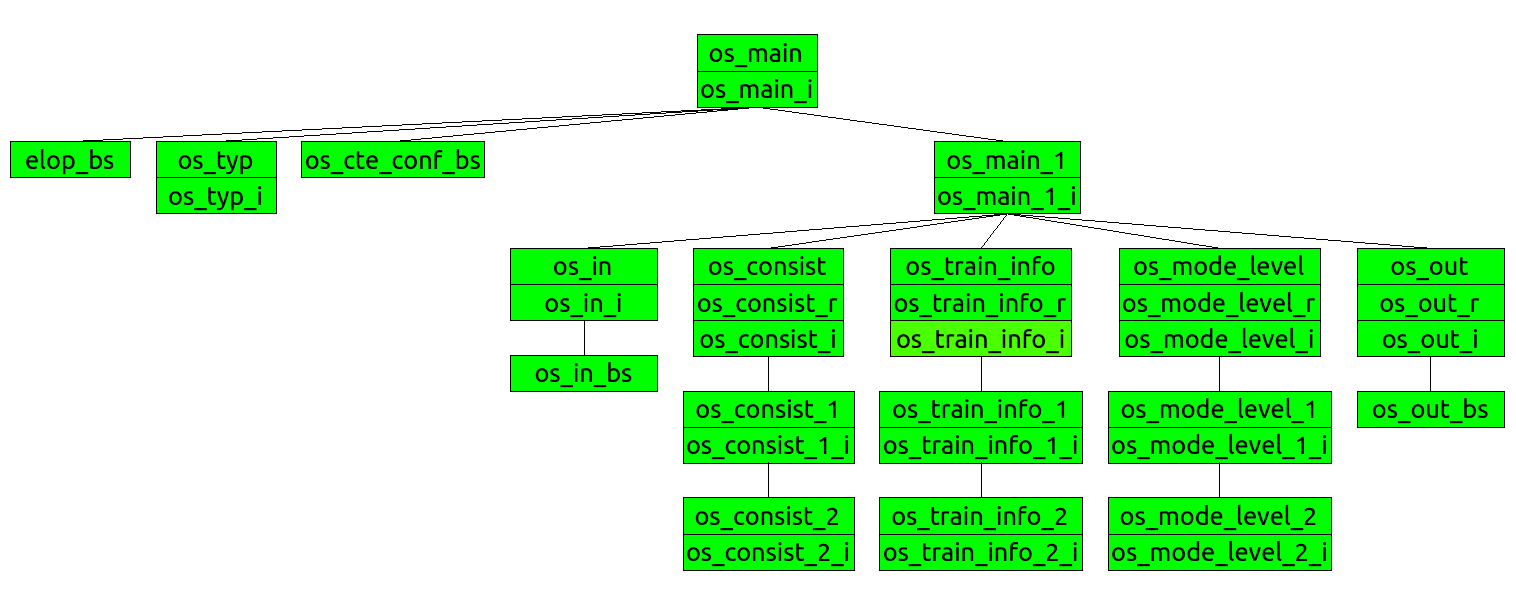
\includegraphics[width=1\textwidth]{procedureos}
\caption{Architecture of the B~model for the Procedure On-Sight example}
\label{fig:procos}
\end{figure}

These three modules are imported by the main sequencer, \verb+os_main_1+, which calls their respective operations. The main sequencer also imports the input module \verb+os_in+, and the output module \verb+os_out+.\\
The typing machine, \verb+os_typ+, and the constant machine, \verb+os_cte_conf_bs+, are both imported by \verb+os_main+, the entry point of the software, which also imports \verb+os_main_1+.\\
 
This ``IMPORTS''-based vertical layout is complemented by a horizontal aspect: the ``SEES'' clause, which enables a component to access another component's data. It is possible for a component to see the components to its left, but not to its right. Thus, a cycle-free graph is maintained.
 
\subsection{Model checking results}
\label{subapp:mc}
ProB has been used on the example model and has shown through model checking that no invariant was violated, and no deadlock state was found. However, for some machines, only a minority of states and nodes have been visited (because of infinite sets in particular) and thus no formal conclusion can be drawn.\\
Additionally, constraint-based checking has also been run and stated, for every operation of every abstract machine, the non-violation of the invariant.

\subsection{Formal proof results}
\label{subapp:proof}
\subsubsection{Project status}
Project status illustrated in figure \ref{fig:atelierb} shows the fully-proved model in Atelier~B.

\begin{figure}[h!]
\centering
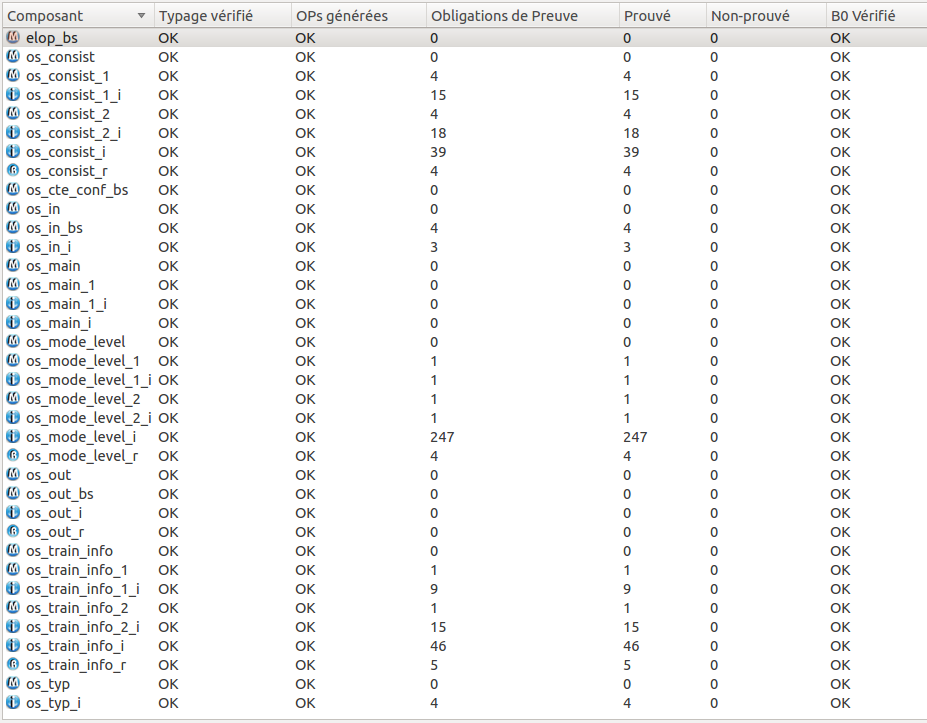
\includegraphics[width=1\textwidth]{atelierb}
\caption{Overview of the B~model in Atelier~B, showing type check, B0 check and proof status}
\label{fig:atelierb}
\end{figure}

This model was proved almost entirely automatically, using the provers with force 0 and force 1. Proving the model results in the certainty of its correctness. In this case, only typing invariants and constraints were expressed, because strong links between the variables do not exist in the example.

\subsubsection{User-defined theories}
When automatic proof fails, the user must provide a manual proof and uses theories for this purpose. Theories are rules that are used to discharge specific goals.\\
In this example, the only module for which interactive proof was required is \verb+os_consist_i+. Below is presented a very simple theory (among several others) used for the proof of this component:

\begin{equation}
\tag{User theory 1}
a < 0 \land 0 \leq b \land 0 < c \Rightarrow a \leq \frac{b}{c}
\end{equation}

This theory is automatically verified by Atelier~B and therefore ensures full consistency of the proof.

\newpage

\begin{thebibliography}{9}
\bibitem{bbook}
	Jean-Raymond Abrial,
	{\itshape The B-Book: Assigning Programs to Meanings},
	Cambridge,
	2005.
\end{thebibliography}

\end{document}



\subsection{Verification and Validation on Event-B models}

The Event-B method share the same language than the classical  B method. Besides both approaches are based on a pre/post -condition mechanism to describe the evolution of the system. Thus similar verification mechanisms can be defined.


\subsubsection{Verification Processes Applicable to Event-B}
\label{sec:verif-proc-appl}

An Event-B model is a formal specification that describes the functional
behavior of a system from a global point of view. In general, an Event-B model
comprises a set of state variables, parametrized events that can modify these
state variables and invariants that describe logical properties thereof.  The
invariants are in first-order predicate logic and can be discharged using
different proof engines, e.g.,\  automatic modern open source SMT solvers and
manual predicate provers.

In general, one starts with a rather abstract description of the model which is
iteratively refined until the desired level of detail is reached. Event-B
supports this refinement by creating the necessary proof obligations that ensure
correct refinement in each step, both for behavioral refinement of events as
well as for data refinement of state variables.

Thanks to the integration into the Eclipse platform, there are many plug-ins
available as extensions. There is a plug-in to use graphical modeling in UML
state machines to describe Event-B models. There is a tight connection to the
ProR requirements engineering plug-in. To facilitate modeling, there are
plug-ins to decompose a model into several sub-models and to facilitate proving
by supporting external formal theories.

Together with the Rodin tool, the Event-B approach was developed in the European
research projects RODIN (2004--2007) and DEPLOY (2008--2012). Since 2011 it is
further developed in the European project ADVANCE\@.

\paragraph{Verification of Type Safety}
\label{sec:verif-type-safety}

Static type checking is a technique that allows the verification of correct
typing for variables at compile / modeling time. It is performed after lexical
and syntactic correctness of the Event-B model have been verified. Static type
checking prevents all type errors at run-time, which eliminates many possible
sources of program errors.

The type system of Event-B is much more expressive than the one of most other
languages, as Event-B also allows the usage of dependent types for variables. In
this case, the type of a variable is dependent of its value, e.g.,\ one can
define the type of all even integers. Event-B can define such types and verify
that events respect the correct dependent typing of variables

In Event-B, every new variable gets a type assigned via a typing invariant. Such
an invariant is either an explicit type assignment or an implicit one, e.g.,\ by
specifying a dependence to another variable which is typed. The integrated type
interference can then deduce the static type of the new variable.

Every event that changes the value of a variable via substitution must also
respect the variable typing. For each event that modifies a variable,  proof
obligations are created that ensure this in a rigorous formal way.

In almost all cases, the proof obligations for type verification are discharged
automatically by the Rodin provers.

\paragraph{Verification of Well-Definedness}
\label{sec:verif-well-defin}

After type checking, one or more well-definedness (WD) proof obligations are
created. This ensures that the expression has a unique meaning and prevents the
usage of expressions that make no sense or are ambiguous.

One prominent example for WD proof obligations in Event-B is the cardinality of
sets. The set of natural numbers $\mathbb{N}$ has countable infinitely many
elements, exactly as many as the set of all even natural numbers
$\mathbb{N}_2:=\{2\cdot n \mid n \in \mathbb{N}\}$. This means that both sets
have the same cardinality, although $\mathbb{N}_2$ is a strict subset of
$\mathbb{N}$.

Therefore, while sets of countable infinite cardinality can be used without any
problem in Event-B models, the usage of cardinality of a set requires the set to
be of finite size which gets verified by an appropriate WD proof obligation.

In almost all cases, the proof obligations for well-definedness are discharged
automatically by the Rodin provers.


\paragraph{Model Simulation}
\label{sec:model-simulation}

A correctly typed Event-B model can be simulated or animated using different
plug-ins like AnimB or ProB. At each step, one of the activated events can be
executed and if applicable parameters for that event can be defined. This allows
for stepping through the formal model, observing the state variables and the
invariants. Using model animation, it is possible to validate the correct
functioning of the model.

\begin{figure}[ht]
  \centering
  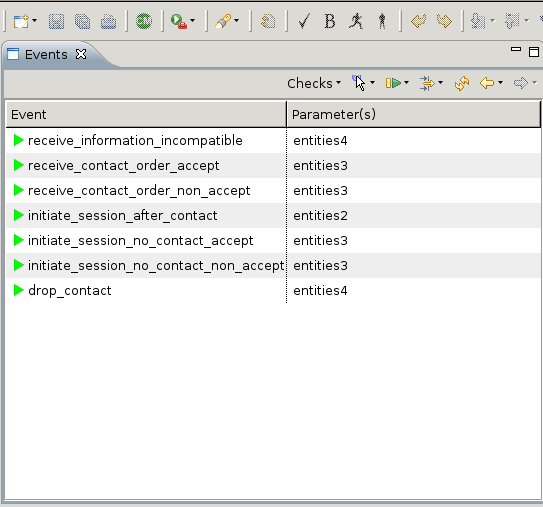
\includegraphics[width=.5\textwidth]{figures/ProBAnimation}
  \caption{ProB Model Animation}
  \label{fig:proBAnimation}
\end{figure}

Figure~\ref{fig:proBAnimation} shows a ProB simulation session. The activated
events are marked green, clicking on them allows for selection of parameters and
to execute the events with the chosen parameters.


\paragraph{Model-Checking of Predicates}
\label{sec:model-check-pred}

Model-checking is a static analysis of the semantics of a model. In general, a
model-checker will create a representation of the whole possible state space of
a model and verify logic properties on this state space. There are many
different possibilities for properties that are verified by model-checkers, some
are listed here:

\begin{itemize}
\item {\bf Equivalence Checking} The equivalence between two models is verified
  given a certain equivalence relation. Often, a specification is compared to
  its (distributed) implementation using bisimulation modulo some reduction
  techniques, e.g.,\ only the externally observable behavior is compared and the
  internal details of the different systems are ignored.
\item {\bf Deadlock Freeness} A deadlock represents a state where the system
  that the system cannot leave as no event is enabled. For a reactive system
  this is always an unwanted state that must be avoided.
\item {\bf Temporal Properties} The evolution of the system over time is
  analyzed, i.e.,\ the admissible event sequences that can lead to different
  states. Roughly, temporal properties comprise \emph{safety properties} which
  describe a set of states that should never be reached and \emph{liveness
    properties} which describe states that should always be reachable. There are
  different temporal logic languages, like LTL and CTL, which allow to describe
  temporal properties of systems.
\end{itemize}

In general, model-checkers suffer from the state space explosion problem. This
means that creating the whole state space becomes often infeasible due to memory
limitations. In general it is also not possible to model-check systems with
infinite state space, like many Event-B models.

In practice, tools like ProB which allow for model-checking of Event-B models,
limit the size of the possible values for variables to a finite subset. While
this means that a correct proof is not possible, it allows for fully automatic
error detection in the model. For any violated property or a deadlock, ProB
provides a counterexample that can be analyzed and therefore allows for
correction of the associated modeling problem.

\begin{figure}[ht]
  \centering
  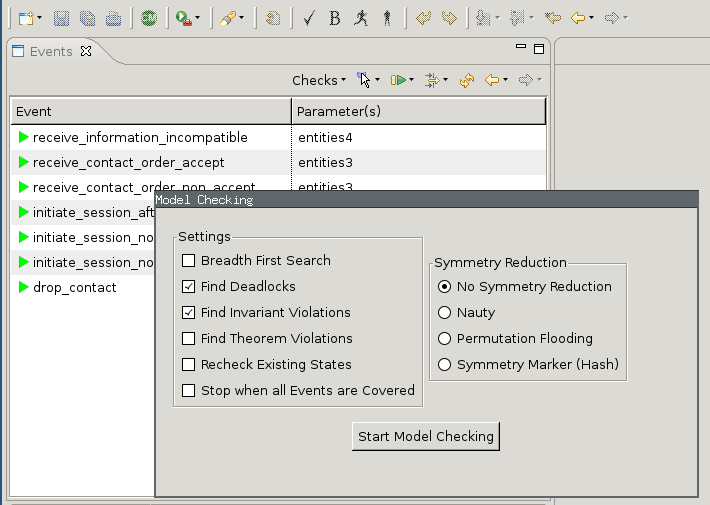
\includegraphics[width=.5\textwidth]{figures/ProBModelChecking}
  \caption{Model-Checking for Deadlocks}
  \label{fig:Prob-model-check}
\end{figure}

Figure~\ref{fig:Prob-model-check} shows the model checking dialog of the Rodin
plug-in for ProB. The currently selected options would check for deadlocks,
i.e.,\ a sequence of events that leads to a situation where no event can be
selected anymore.


\paragraph{Formal Proof of Predicates}
\label{sec:form-proof-pred}

Formal proof techniques provide a much more powerful way to verify predicates
than model-checking. Instead of the creation of the full state-space, they use a
proof calculus to iteratively simplify predicates and to reduce them onto known
lemmas or axioms, thus discharging them.

In contrast to model-checking, formal proof is applicable to models of infinite
size and can cope with undecidable problems. Although this means that there
sometimes will be a manual step in a proof, there are many automated tools that
support formal proofs and can often discharge proof obligations without any
manual intervention.

The Rodin platform natively supports manual construction of formal proofs by
allowing easy access and manipulation of the proof tree and predicate
hypotheses. It also provides access to different automated provers, i.e.,\ the
free of charge AtelierB provers, an open source SMT plug-in that supports
several solvers\footnote{supported open source SMT solvers include: verIT,
  Alt-Ergo, CVC3, Z3} as well as an open source plug-in that connects Rodin to
the Isabelle/HOL proof assistant.

\begin{figure}[ht]
  \centering
  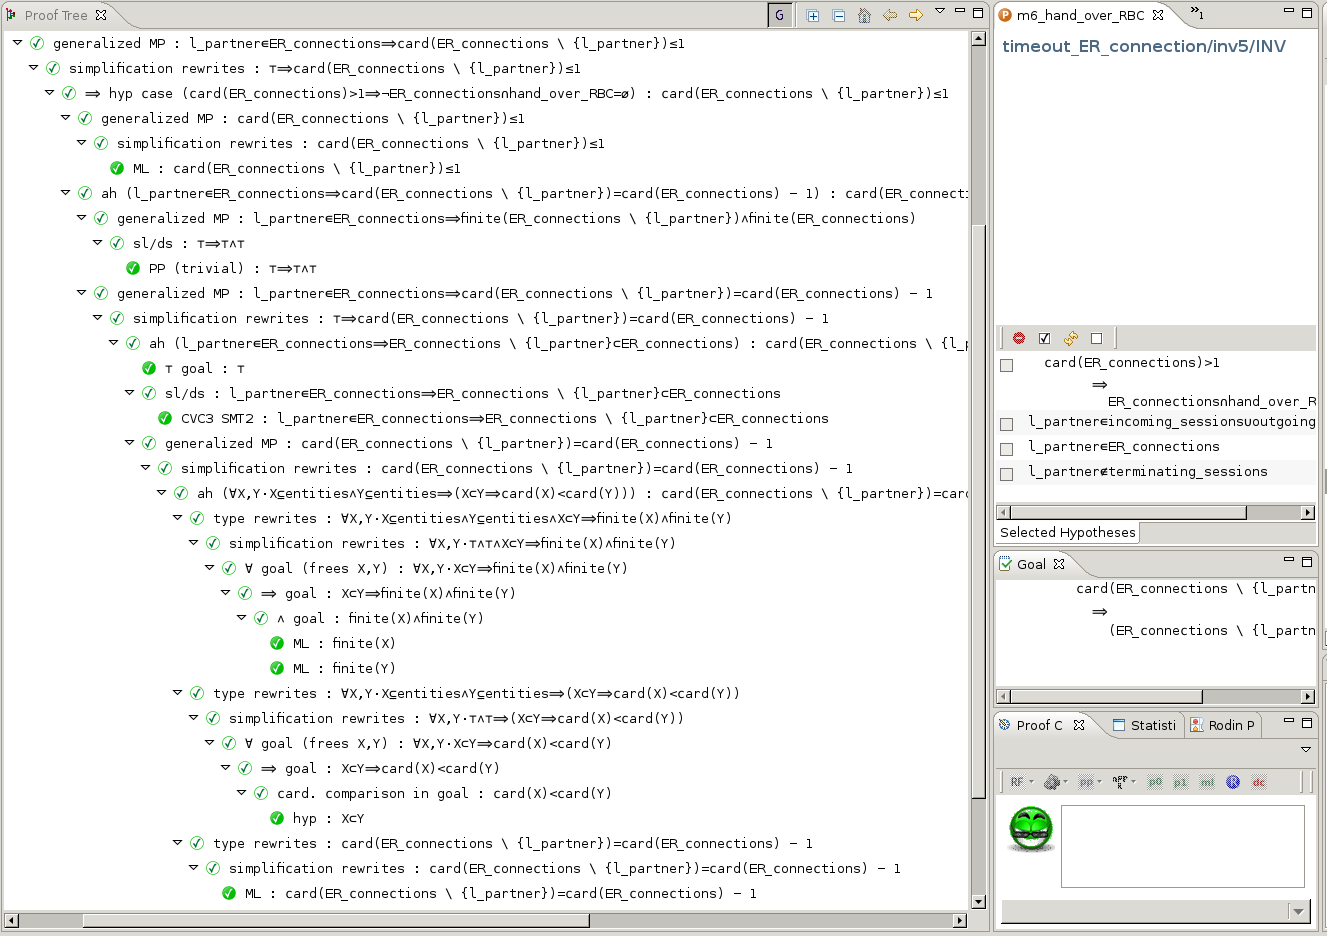
\includegraphics[width=1\textwidth]{figures/ProofTree}
  \caption{Rodin Proof Tree}
  \label{fig:proof-tree}
\end{figure}

Figure~\ref{fig:proof-tree} shows a part of a Rodin proof tree for an
invariant. Its green color signals that the proof is finished, at each node in
the tree, the applied proof rule is shown. This allows for easy inspection of
the proofs and allows both for humans and for machines to verify the correctness
of the proof steps.


\paragraph{Verification of Refinement Correctness}
\label{sec:verif-refin-corr}

Rodin provides extensive support for a top-down development approach and allows
for an iterative refinement of models. The model is developed using different
levels of detail, starting from a rather abstract view, refining the details
where necessary or desired. This refinement process can either be applied to
the events or the variables.

\subparagraph{Data Refinement}
\label{sec:data-refinement}

In general, a data refinement replaces a variable with another one, or multiple
other ones. For example a Boolean variable in the abstract model is replaces by
an enumeration with different possible values. To ensure a correct refinement,
one has to manually supply a ``gluing'' invariant that describes the connection
of the refined and the abstract variable. For example one subset of the possible
values for the enumeration in the refined model would correspond to a value of
``True'' in the abstract model, the remaining values of the enumeration to a
value ``False''. The abstract variable is then deleted from the refined model,
and the necessary proof obligations are created automatically by Rodin.


\subparagraph{Code Refinement}
\label{sec:code-refinement}

For event (or code) refinement, Rodin automatically creates the necessary proof
obligations that ensure that the abstract system is correctly refined by the
more detailed model. This includes the verification that each refining event
only modifies variables that are also modified by the abstract event and that
the modification is equivalent. It also includes verification of guard
strengthening, i.e.,\ the guards of a refining event must be at least as
constraining as of the refined abstract event. A common code refinement is to
split an event in several more specialized ones, where the additional guards
ensure mutual exclusion of the activation conditions.

\begin{figure}[ht]
  \centering
  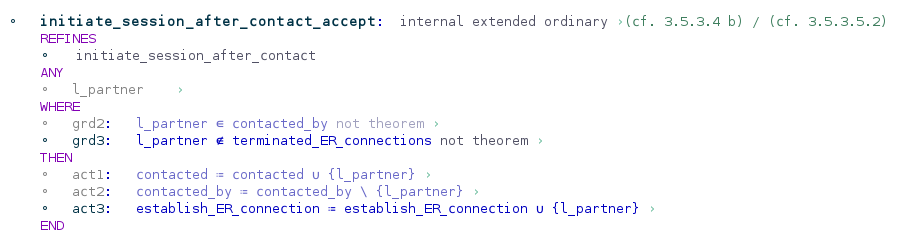
\includegraphics[width=.9\textwidth]{figures/EventRefine}
  \caption{Event Refinement}
  \label{fig:event-refine}
\end{figure}

Figure~\ref{fig:event-refine} shows a refining event with guard strengthening
and an additional variable that is modified. The pale blue colored guards and
actions are derived from the refined event, the darker colored guard and action
are the additional ones for the refining event.


\paragraph{Verification of Design Step Requirements}
\label{sec:verif-design-step}

This section reports on the verification activities of the correct
implementation of the design step requirements. The goal of the activity is to
establish a correct formal representation of the design step requirements.

The activity is described in the Verification and Validation
Plan~\cite{vnvplan}.  In short, it consists of formalizing and proving the
identified requirements of a preceding phase, to ensure their correct
implementation of the requirements. To achieve this, we use the direct
connection of the Event-B model with the ProR based on an EMF model of the
Event-B model.


\paragraph{Verification of Safety Requirements}
\label{sec:verif-safety-requ}

A safety analysis identifies additional requirements which guarantee the safety
of a system. It must be verified that the system model correctly implements
these non-functional requirements. Not every safety requirement is applicable on
the system development level. Many are on the implementation level, e.g.,\ they
demand that certain safety-critical functions are done in a redundant way to
reduce the risk of malfunctioning or loss of that function.

In the safety analysis~\cite{safetyBrice}, a list of safety requirements was
identified using an FMEA analysis of the communication system. A ReqIf file
captures all these safety requirements within ProR, the concerned functional
requirements are traced in the ReqIf file for SS~026 section 3.5.

Each of the safety requirements is examined for applicability in the system
level model, the identified ones are formalized. Most often, the safety
requirements are represented as one or more additional invariants in the system
model. These invariants are linked to the ReqIf file that describes the safety
requirements, ensuring traceability in the model.

\begin{figure}[ht]
  \centering
  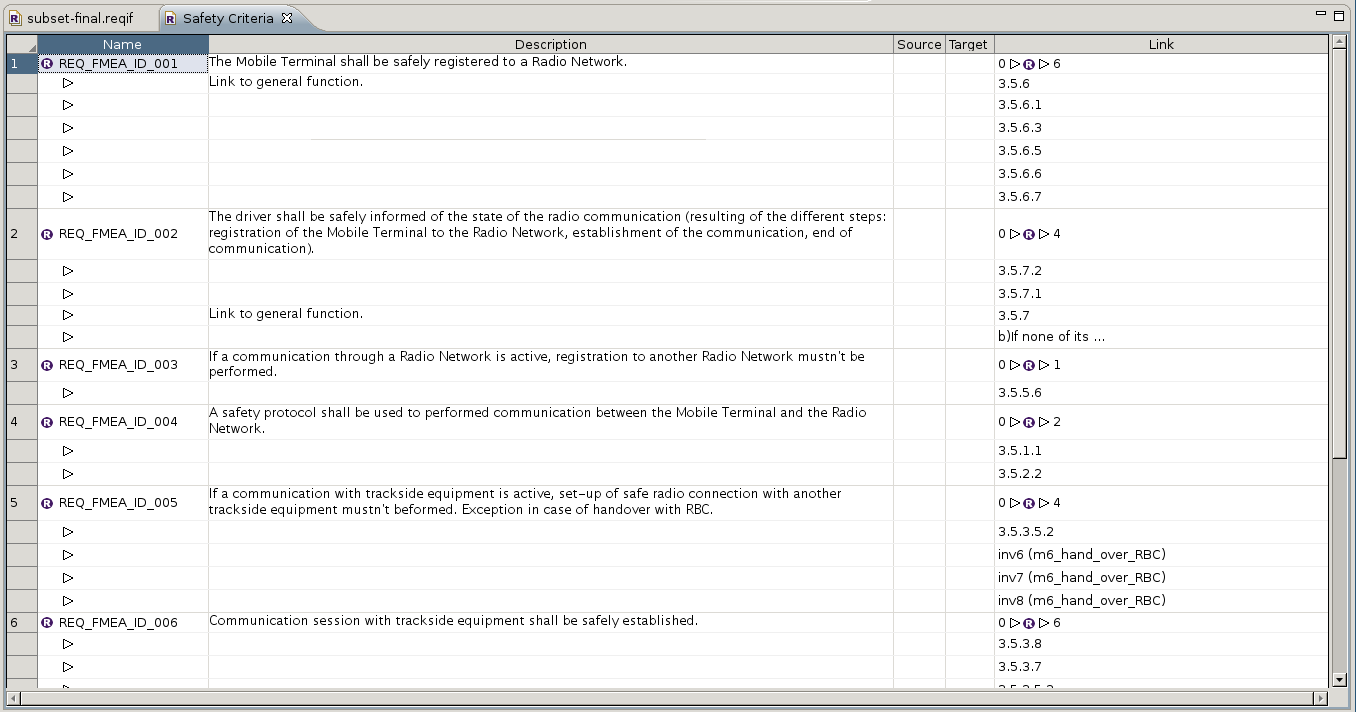
\includegraphics[width=1\textwidth]{figures/ProRSafetyReq}
  \caption{Safety Requirements}
  \label{fig:pror-safety-req}
\end{figure}

Figure~\ref{fig:pror-safety-req} shows a ReqIf document in Rodin (via the ProR
plug-in) which holds the safety requirements defined by the safety analysis. For
each requirement, there are references to the concerned elements of SS~026 and
to Event-B elements where applicable, e.g.,\ {\sf REQ\_FMEA\_ID\_005} which is
linked to the invariants, {\sf inv6}, {\sf inv7} and {\sf inv8}.


\paragraph{Verification of Requirements Coverage}
\label{sec:verif-requ-cover}

This section reports on the verification activities of the coverage of the
design step requirements. The goal of the activity is to establish the coverage
degree of the formal representation of the design step requirements.

The activity is described in the Verification and Validation
Plan~\cite{vnvplan}.  In short, in consists of analyzing the coverage of the
identified requirements of a preceding phase, to ensure their completeness of
implementation of the requirements wrt.\ the refinement level of the model. To
achieve this, we use the direct connection of the Event-B model with the ProR
based on an EMF model of the Event-B model.


\subsubsection{Object of Verification}
\label{sec:object-verification}

The object of verification is the Event-B model for the communication
establishing\footnote{\url{https://github.com/openETCS/model-evaluation/tree/master/model/Event_B_Systerel/Subset_026_comm_session}}. It
is from the strictly formal modeling phase and represents the communication
session management of the OBU\@.

\paragraph{Available Specification}
\label{sec:avail-spec}

The model implements the requirements for the communication session management
as described in SS~026, section 3.5\cite{subset-26}.

This section describes the establishing, maintaining and termination of a
communication session of the OBU with on-track systems.

%\subsubsection{Detailed verification plan}
%\label{sec:deta-verif-plan}

\paragraph{Goals}

One goal is the development of a strictly formal, fully proven model of the
communication session management and to provide evidence of covering the
necessary requirements of SS~026 as well as proving correctness of the model
wrt.\ the requirements ans attaining a good coverage of the model wrt.\ the
requirements.

The second goal is to correctly implement the applicable safety requirements
identified by the safety analysis. Both functional and safety requirements
should be traced in the model and a requirement document in a standardized
format.

The formal model will represent the described functionality on the system level,
the correct functioning can be validated by step-wise simulation and
model-checking of deadlock-freeness.


\paragraph{Method/Approach}
\label{sec:methodapproach}

At first, the basic functionality described in the section 3.5 that are
identified. These serve as basis for a first abstract model, which is refined
iteratively, adding the desired level of detail. The elements of SS~026 are
traced using links from Event-B to the ProR file in ReqIf format. Requirements
are formalized as invariants and proven where applicable.

\paragraph{Means}
\label{sec:means}

The means used are:
\begin{itemize}
\item open source Rodin tool (\url{http://www.event-b.org/}), including plug-ins
  (for details
  see~\url{https://github.com/openETCS/model-evaluation/blob/master/model/Event_B_Systerel/Subset_026_comm_session/latex/subset_3_5.pdf})
\item ProR requirements modeling tool~\url{http://www.pror.org}
\item open source ProB model checker and B model
  simulator~\url{http://www.stups.uni-duesseldorf.de/ProB/index.php5/Main_Page}
\item open source CVC3 (\url{http://www.cs.nyu.edu/acsys/cvc3/}), verIT
  (\url{www.verit-solver.org}) and Alt-Ergo (\url{http://alt-ergo.lri.fr}) SMT
  solvers
\end{itemize}

% \subparagraph{Other}

%  \bgcmmnt{optional, might be renamed}

\paragraph{Results}
\label{sec:results}

\begin{itemize}
\item The result is a fully formal model of the communication session management
  as described in section 3.5 of SS~026.
\item Each implemented element of this section is linked to the ProR
  requirements file, both specification elements that describe how something has
  to be done, as well as requirements that describe what must be achieved.
\item The model can be simulated / animated, either with the AnimB or the ProB
  plug-in, validating the functional capabilities.
\item The requirements are formalized as invariants in predicate logic, their
  proofs are for the most part fully automatic.
\item It was found that while the SS~026 communication management explicitly
  allows multiple communication partners (see RBC handover), there is no
  explicit limit of established communication connections given in section 3.5.
\item A complete covering of the elements of SS~026 was not realized, e.g.,\
  there is a representation of the contents of a message, but its explicit
  format is not implemented. This is considered an implementation detail without
  influence for a system level analysis. In general, Event-B models will not be
  refined up to the implementation level.
\end{itemize}

\paragraph{Summary}

The created fully formal functional model allows for formalization and proof of
SS~026 requirements. The integration of Rodin into Eclipse provides easy access
to extensions like the ProR requirements tool which allows for validation of
coverage of requirements.

The integration of various provers, in particular the SMT plug-in automates a
large part of the formal verification. For the model of the communication
management, from 382 non-trivial\footnote{many WD proof obligations are so
  trivial that they will not be shown in Rodin} proof obligations, only 12,
i.e.,\ $3.2\%$ require any manual intervention.

\paragraph{Evidence produced}
\label{sec:evidence-produced}

The formal Event-B model, including a ReqIf document for section 3.5 of SS~026
and a pdf documentation of the model can be found at
\url{https://github.com/openETCS/model-evaluation/tree/master/model/Event_B_Systerel/Subset_026_comm_session}

\subsubsection{Conclusions/Lessons learned}

Having an abstract formal model of the implemented functionality which can be
simulated, allows for interesting insights into the overall functioning of a
system. Formalized requirements are very helpful in both the identification of
ambiguous requirements and in their clarification.

The elements of SS~026 are of very different nature. Some describe rather
low-level specification details, other describe ``real'' requirements. Without
an analysis as done with this Event-B model, it can be difficult to decide which
elements must be considered on a system level analysis and which on the lower
implementation level.


\subsubsection{Future Activities}
\label{sec:future-activities}

For other sections of SS~026, that describe a functionality in a way that can be
captured in an iteratively refined model and which has interesting requirements
on a rather high level, creating an Event-B model can provide insight into the
functioning, identify ambiguous or erroneous elements in the specification and
can provide the basis for logical pre- and post conditions of the later
implementation.



\subsection{Verification processes applicable to a\\SCADE~model}

The verifier shall be independent and shall neither be Requirements Manager, Designer nor Implementer as defined in the safety standards EN 50128 v2011.

The input documents needed are all the necessary System and Software Documentation used for the SCADE design activity and all the documentation produced during this phase, such as the SCADE Design Description, the SCADE Design Test Specification and the SCADE Design Test Report.

\subsubsection{Respect of modelling rules}

Syntactic rules of SCADE language are verified with the Quick Check tool available in the publisher. If an error is detected it must be corrected or justified in the SCADE Design Description document by the designer. The verifier shall ensure that no error remains or the justification associated is correct.

For specific modelling rules the verification has to be made manually by the verifier and described in the Verification Report. A grid of verification may be created in order to prove the compliance of the model with the rules. On some cases, dedicated tools can be developed.

\subsubsection{Specification traceability check}

The verification of the compliance of the SCADE model with each requirement has to be made manually, by the verifier. 

The Scade model shall be correct according to the informal requirements and the informal specification shall be completely covered : each specification requirement must be traced in the SCADE model. The specification requirements which are not covered by the SCADE model must be listed and justified in the SCADE Design Description document by the designer.

\subsubsection{Testing and Validation of the model}

The verifier shall control the activity of software testing performed by the tester.

The software testing uses the Model Test Coverage (MTC) and the Generic Qualified Testing Environment (QTE) tools from SCADE. Five steps are performed.
\begin{itemize}
\item Establish the Test Specification document.
\item Writing scenarios in order to test the different functions independently.
\item Running scenarios on the SCADE model.
\item Extraction and analysis of results and the associated coverage.
\item Establish the Test Report.
\end{itemize}

\subsection{Results}

All these different verifications activities shall be described in the Verification and Validation Plan, and their results shall be record in a Verification Report. Each disparity must be corrected or justified.

\subsubsection{Verification report content}

The verifier shall produce a Verification Report containing the proof of the compliance of the SCADE model. It shall include the following points:
\begin{itemize}
\item the identity, version and configuration of SCADE model;
\item the verifier name;
\item the goal of the Verification Report;
\item the result of each verification process with:
\subitem - items which do not conform to the specifications;
\subitem - components, data, structures and algorithms poorly adapted to the problem;
\subitem - detected errors or deficiencies.
\item the fulfilment of, or deviation from, the Software Verification Plan;
\item assumptions if any;
\item a summary of the verification results.
\end{itemize}

\subsection{Conclusion}

The use of SCADE with its verification processes is compliant with the CENELEC norm but as it is not developed as open-source it is not compliant with the goal of openETCs project. 



\nocite{*}
%===================================================
%Do NOT change anything below this line

%\bibliographystyle{IEEEtran}
\bibliographystyle{unsrt}

\bibliography{biblio}
%

\end{document}
